%!TEX root = ../blob1.tex

\def\xxpar#1#2{\smallskip\noindent{\bf #1} {\it #2} \smallskip}
\def\mmpar#1#2#3{\smallskip\noindent{\bf #1} (#2). {\it #3} \smallskip}

\section{$n$-categories and their modules}
\label{sec:ncats}

\subsection{Definition of $n$-categories}
\label{ss:n-cat-def}

Before proceeding, we need more appropriate definitions of $n$-categories, 
$A_\infty$ $n$-categories, modules for these, and tensor products of these modules.
(As is the case throughout this paper, by ``$n$-category" we mean some notion of
a ``weak" $n$-category with ``strong duality".)

The definitions presented below tie the categories more closely to the topology
and avoid combinatorial questions about, for example, the minimal sufficient
collections of generalized associativity axioms; we prefer maximal sets of axioms to minimal sets.
For examples of topological origin
(e.g.\ categories whose morphisms are maps into spaces or decorated balls), 
it is easy to show that they
satisfy our axioms.
For examples of a more purely algebraic origin, one would typically need the combinatorial
results that we have avoided here.

\medskip

There are many existing definitions of $n$-categories, with various intended uses.
In any such definition, there are sets of $k$-morphisms for each $0 \leq k \leq n$.
Generally, these sets are indexed by instances of a certain typical shape. 
Some $n$-category definitions model $k$-morphisms on the standard bihedron (interval, bigon, and so on).
Other definitions have a separate set of 1-morphisms for each interval $[0,l] \sub \r$, 
a separate set of 2-morphisms for each rectangle $[0,l_1]\times [0,l_2] \sub \r^2$,
and so on.
(This allows for strict associativity.)
Still other definitions (see, for example, \cite{MR2094071})
model the $k$-morphisms on more complicated combinatorial polyhedra.

For our definition, we will allow our $k$-morphisms to have any shape, so long as it is homeomorphic to the standard $k$-ball.
Thus we associate a set of $k$-morphisms $\cC_k(X)$ to any $k$-manifold $X$ homeomorphic 
to the standard $k$-ball.
By ``a $k$-ball" we mean any $k$-manifold which is homeomorphic to the 
standard $k$-ball.
We {\it do not} assume that it is equipped with a 
preferred homeomorphism to the standard $k$-ball, and the same applies to ``a $k$-sphere" below.

Given a homeomorphism $f:X\to Y$ between $k$-balls (not necessarily fixed on 
the boundary), we want a corresponding
bijection of sets $f:\cC(X)\to \cC(Y)$.
(This will imply ``strong duality", among other things.) Putting these together, we have

\begin{axiom}[Morphisms]
\label{axiom:morphisms}
For each $0 \le k \le n$, we have a functor $\cC_k$ from 
the category of $k$-balls and 
homeomorphisms to the category of sets and bijections.
\end{axiom}


(Note: We usually omit the subscript $k$.)

We are being deliberately vague about what flavor of $k$-balls
we are considering.
They could be unoriented or oriented or Spin or $\mbox{Pin}_\pm$.
They could be topological or PL or smooth.
%\nn{need to check whether this makes much difference}
(If smooth, ``homeomorphism" should be read ``diffeomorphism", and we would need
to be fussier about corners and boundaries.)
For each flavor of manifold there is a corresponding flavor of $n$-category.
For simplicity, we will concentrate on the case of PL unoriented manifolds.

(The ambitious reader may want to keep in mind two other classes of balls.
The first is balls equipped with a map to some other space $Y$ (c.f. \cite{MR2079378}). 
This will be used below to describe the blob complex of a fiber bundle with
base space $Y$.
The second is balls equipped with a section of the tangent bundle, or the frame
bundle (i.e.\ framed balls), or more generally some flag bundle associated to the tangent bundle.
These can be used to define categories with less than the ``strong" duality we assume here,
though we will not develop that idea fully in this paper.)

Next we consider domains and ranges of morphisms (or, as we prefer to say, boundaries
of morphisms).
The 0-sphere is unusual among spheres in that it is disconnected.
Correspondingly, for 1-morphisms it makes sense to distinguish between domain and range.
(Actually, this is only true in the oriented case, with 1-morphisms parameterized
by {\it oriented} 1-balls.)
For $k>1$ and in the presence of strong duality the division into domain and range makes less sense.
For example, in a pivotal tensor category, there are natural isomorphisms $\Hom{}{A}{B \tensor C} \isoto \Hom{}{B^* \tensor A}{C}$, etc. 
(sometimes called ``Frobenius reciprocity''), which canonically identify all the morphism spaces which have the same boundary.
We prefer to not make the distinction in the first place.

Instead, we will combine the domain and range into a single entity which we call the 
boundary of a morphism.
Morphisms are modeled on balls, so their boundaries are modeled on spheres.
In other words, we need to extend the functors $\cC_{k-1}$ from balls to spheres, for 
$1\le k \le n$.
At first it might seem that we need another axiom for this, but in fact once we have
all the axioms in this subsection for $0$ through $k-1$ we can use a colimit
construction, as described in \S\ref{ss:ncat-coend} below, to extend $\cC_{k-1}$
to spheres (and any other manifolds):

\begin{lem}
\label{lem:spheres}
For each $1 \le k \le n$, we have a functor $\cl{\cC}_{k-1}$ from 
the category of $k{-}1$-spheres and 
homeomorphisms to the category of sets and bijections.
\end{lem}

We postpone the proof of this result until after we've actually given all the axioms.
Note that defining this functor for some $k$ only requires the data described in Axiom \ref{axiom:morphisms} at level $k$, 
along with the data described in the other axioms at lower levels. 

%In fact, the functors for spheres are entirely determined by the functors for balls and the subsequent axioms. (In particular, $\cC(S^k)$ is the colimit of $\cC$ applied to decompositions of $S^k$ into balls.) However, it is easiest to think of it as additional data at this point.

\begin{axiom}[Boundaries]\label{nca-boundary}
For each $k$-ball $X$, we have a map of sets $\bd: \cC_k(X)\to \cl{\cC}_{k-1}(\bd X)$.
These maps, for various $X$, comprise a natural transformation of functors.
\end{axiom}

(Note that the first ``$\bd$" above is part of the data for the category, 
while the second is the ordinary boundary of manifolds.)

Given $c\in\cl{\cC}(\bd(X))$, we will write $\cC(X; c)$ for $\bd^{-1}(c)$, those morphisms with specified boundary $c$.

Most of the examples of $n$-categories we are interested in are enriched in the following sense.
The various sets of $n$-morphisms $\cC(X; c)$, for all $n$-balls $X$ and
all $c\in \cl{\cC}(\bd X)$, have the structure of an object in some auxiliary symmetric monoidal category
(e.g.\ vector spaces, or modules over some ring, or chain complexes),
\nn{actually, need both disj-union/sub and product/tensor-product; what's the name for this sort of cat?}
and all the structure maps of the $n$-category should be compatible with the auxiliary
category structure.
Note that this auxiliary structure is only in dimension $n$;
$\cC(Y; c)$ is just a plain set if $\dim(Y) < n$.

\medskip

(In order to simplify the exposition we have concentrated on the case of 
unoriented PL manifolds and avoided the question of what exactly we mean by 
the boundary a manifold with extra structure, such as an oriented manifold.
In general, all manifolds of dimension less than $n$ should be equipped with the germ
of a thickening to dimension $n$, and this germ should carry whatever structure we have 
on $n$-manifolds.
In addition, lower dimensional manifolds should be equipped with a framing
of their normal bundle in the thickening; the framing keeps track of which
side (iterated) bounded manifolds lie on.
For example, the boundary of an oriented $n$-ball
should be an $n{-}1$-sphere equipped with an orientation of its once stabilized tangent
bundle and a choice of direction in this bundle indicating
which side the $n$-ball lies on.)

\medskip

We have just argued that the boundary of a morphism has no preferred splitting into
domain and range, but the converse meets with our approval.
That is, given compatible domain and range, we should be able to combine them into
the full boundary of a morphism.
The following lemma will follow from the colimit construction used to define $\cl{\cC}_{k-1}$
on spheres.

\begin{lem}[Boundary from domain and range]
\label{lem:domain-and-range}
Let $S = B_1 \cup_E B_2$, where $S$ is a $k{-}1$-sphere $(1\le k\le n)$,
$B_i$ is a $k{-}1$-ball, and $E = B_1\cap B_2$ is a $k{-}2$-sphere (Figure \ref{blah3}).
Let $\cC(B_1) \times_{\cl{\cC}(E)} \cC(B_2)$ denote the fibered product of the 
two maps $\bd: \cC(B_i)\to \cl{\cC}(E)$.
Then we have an injective map
\[
	\gl_E : \cC(B_1) \times_{\cl{\cC}(E)} \cC(B_2) \into \cl{\cC}(S)
\]
which is natural with respect to the actions of homeomorphisms.
(When $k=1$ we stipulate that $\cl{\cC}(E)$ is a point, so that the above fibered product
becomes a normal product.)
\end{lem}

\begin{figure}[!ht]
$$
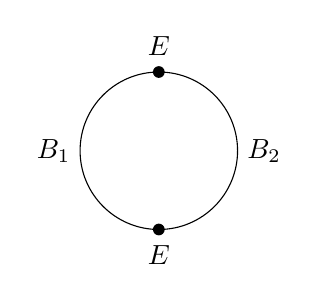
\begin{tikzpicture}[%every label/.style={green}
]
\node[fill=black, circle, label=below:$E$, inner sep=1.5pt](S) at (0,0) {};
\node[fill=black, circle, label=above:$E$, inner sep=1.5pt](N) at (0,2) {};
\draw (S) arc  (-90:90:1);
\draw (N) arc  (90:270:1);
\node[left] at (-1,1) {$B_1$};
\node[right] at (1,1) {$B_2$};
\end{tikzpicture}
$$
\caption{Combining two balls to get a full boundary.}\label{blah3}\end{figure}

Note that we insist on injectivity above. 
The lemma follows from Definition \ref{def:colim-fields} and Lemma \ref{lem:colim-injective}.

Let $\cl{\cC}(S)_E$ denote the image of $\gl_E$.
We will refer to elements of $\cl{\cC}(S)_E$ as ``splittable along $E$" or ``transverse to $E$". 

If $X$ is a $k$-ball and $E \sub \bd X$ splits $\bd X$ into two $k{-}1$-balls $B_1$ and $B_2$
as above, then we define $\cC(X)_E = \bd^{-1}(\cl{\cC}(\bd X)_E)$.

We will call the projection $\cl{\cC}(S)_E \to \cC(B_i)$
a {\it restriction} map and write $\res_{B_i}(a)$
(or simply $\res(a)$ when there is no ambiguity), for $a\in \cl{\cC}(S)_E$.
More generally, we also include under the rubric ``restriction map" the
the boundary maps of Axiom \ref{nca-boundary} above,
another class of maps introduced after Axiom \ref{nca-assoc} below, as well as any composition
of restriction maps.
In particular, we have restriction maps $\cC(X)_E \to \cC(B_i)$
($i = 1, 2$, notation from previous paragraph).
These restriction maps can be thought of as 
domain and range maps, relative to the choice of splitting $\bd X = B_1 \cup_E B_2$.


Next we consider composition of morphisms.
For $n$-categories which lack strong duality, one usually considers
$k$ different types of composition of $k$-morphisms, each associated to a different direction.
(For example, vertical and horizontal composition of 2-morphisms.)
In the presence of strong duality, these $k$ distinct compositions are subsumed into 
one general type of composition which can be in any ``direction".

\begin{axiom}[Composition]
Let $B = B_1 \cup_Y B_2$, where $B$, $B_1$ and $B_2$ are $k$-balls ($0\le k\le n$)
and $Y = B_1\cap B_2$ is a $k{-}1$-ball (Figure \ref{blah5}).
Let $E = \bd Y$, which is a $k{-}2$-sphere.
Note that each of $B$, $B_1$ and $B_2$ has its boundary split into two $k{-}1$-balls by $E$.
We have restriction (domain or range) maps $\cC(B_i)_E \to \cC(Y)$.
Let $\cC(B_1)_E \times_{\cC(Y)} \cC(B_2)_E$ denote the fibered product of these two maps. 
We have a map
\[
	\gl_Y : \cC(B_1)_E \times_{\cC(Y)} \cC(B_2)_E \to \cC(B)_E
\]
which is natural with respect to the actions of homeomorphisms, and also compatible with restrictions
to the intersection of the boundaries of $B$ and $B_i$.
If $k < n$ we require that $\gl_Y$ is injective.
(For $k=n$, see below.)
\end{axiom}

\begin{figure}[!ht]
$$
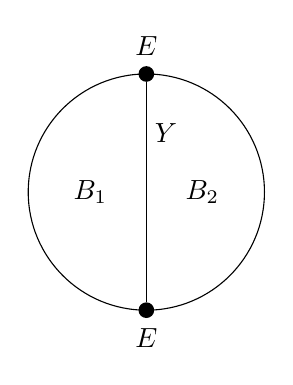
\begin{tikzpicture}[%every label/.style={green},
				x=1.5cm,y=1.5cm]
\node[fill=black, circle, label=below:$E$, inner sep=2pt](S) at (0,0) {};
\node[fill=black, circle, label=above:$E$, inner sep=2pt](N) at (0,2) {};
\draw (S) arc  (-90:90:1);
\draw (N) arc  (90:270:1);
\draw (N) -- (S);
\node[left] at (-1/4,1) {$B_1$};
\node[right] at (1/4,1) {$B_2$};
\node at (1/6,3/2)  {$Y$};
\end{tikzpicture}
$$
\caption{From two balls to one ball.}\label{blah5}\end{figure}

\begin{axiom}[Strict associativity] \label{nca-assoc}
The composition (gluing) maps above are strictly associative.
Given any splitting of a ball $B$ into smaller balls $B_1,\ldots,B_m$, 
any sequence of gluings of the smaller balls yields the same result.
\end{axiom}

\begin{figure}[!ht]
$$\mathfig{.65}{ncat/strict-associativity}$$
\caption{An example of strict associativity.}\label{blah6}\end{figure}

We'll use the notations  $a\bullet b$ as well as $a \cup b$ for the glued together field $\gl_Y(a, b)$.
In the other direction, we will call the projection from $\cC(B)_E$ to $\cC(B_i)_E$ 
a restriction map (one of many types of map so called) and write $\res_{B_i}(a)$ for $a\in \cC(B)_E$.
%Compositions of boundary and restriction maps will also be called restriction maps.
%For example, if $B$ is a $k$-ball and $Y\sub \bd B$ is a $k{-}1$-ball, there is a
%restriction map from $\cC(B)_{\bd Y}$ to $\cC(Y)$.

We will write $\cC(B)_Y$ for the image of $\gl_Y$ in $\cC(B)$.
We will call elements of $\cC(B)_Y$ morphisms which are 
``splittable along $Y$'' or ``transverse to $Y$''.
We have $\cC(B)_Y \sub \cC(B)_E \sub \cC(B)$.

More generally, let $\alpha$ be a subdivision of a ball $X$ into smaller balls.
Let $\cC(X)_\alpha \sub \cC(X)$ denote the image of the iterated gluing maps from 
the smaller balls to $X$.
We  say that elements of $\cC(X)_\alpha$ are morphisms which are ``splittable along $\alpha$".
In situations where the subdivision is notationally anonymous, we will write
$\cC(X)\spl$ for the morphisms which are splittable along (a.k.a.\ transverse to)
the unnamed subdivision.
If $\beta$ is a subdivision of $\bd X$, we define $\cC(X)_\beta \deq \bd\inv(\cl{\cC}(\bd X)_\beta)$;
this can also be denoted $\cC(X)\spl$ if the context contains an anonymous
subdivision of $\bd X$ and no competing subdivision of $X$.

The above two composition axioms are equivalent to the following one,
which we state in slightly vague form.

\xxpar{Multi-composition:}
{Given any decomposition $B = B_1\cup\cdots\cup B_m$ of a $k$-ball
into small $k$-balls, there is a 
map from an appropriate subset (like a fibered product) 
of $\cC(B_1)\spl\times\cdots\times\cC(B_m)\spl$ to $\cC(B)\spl$,
and these various $m$-fold composition maps satisfy an
operad-type strict associativity condition (Figure \ref{fig:operad-composition}).}

\begin{figure}[!ht]
$$\mathfig{.8}{ncat/operad-composition}$$
\caption{Operad composition and associativity}\label{fig:operad-composition}\end{figure}

The next axiom is related to identity morphisms, though that might not be immediately obvious.

\begin{axiom}[Product (identity) morphisms, preliminary version]
For each $k$-ball $X$ and $m$-ball $D$, with $k+m \le n$, there is a map $\cC(X)\to \cC(X\times D)$, 
usually denoted $a\mapsto a\times D$ for $a\in \cC(X)$.
These maps must satisfy the following conditions.
\begin{enumerate}
\item
If $f:X\to X'$ and $\tilde{f}:X\times D \to X'\times D'$ are homeomorphisms such that the diagram
\[ \xymatrix{
	X\times D \ar[r]^{\tilde{f}} \ar[d]_{\pi} & X'\times D' \ar[d]^{\pi} \\
	X \ar[r]^{f} & X'
} \]
commutes, then we have 
\[
	\tilde{f}(a\times D) = f(a)\times D' .
\]
\item
Product morphisms are compatible with gluing (composition) in both factors:
\[
	(a'\times D)\bullet(a''\times D) = (a'\bullet a'')\times D
\]
and
\[
	(a\times D')\bullet(a\times D'') = a\times (D'\bullet D'') .
\]
\item
Product morphisms are associative:
\[
	(a\times D)\times D' = a\times (D\times D') .
\]
(Here we are implicitly using functoriality and the obvious homeomorphism
$(X\times D)\times D' \to X\times(D\times D')$.)
\item
Product morphisms are compatible with restriction:
\[
	\res_{X\times E}(a\times D) = a\times E
\]
for $E\sub \bd D$ and $a\in \cC(X)$.
\end{enumerate}
\end{axiom}

We will need to strengthen the above preliminary version of the axiom to allow
for products which are ``pinched" in various ways along their boundary.
(See Figure \ref{pinched_prods}.)
\begin{figure}[t]
$$
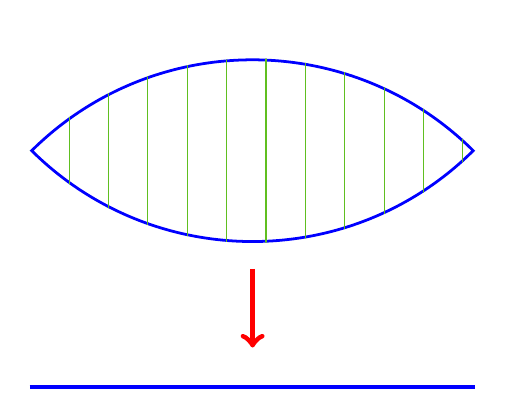
\begin{tikzpicture}[baseline=0]
\begin{scope}
\path[clip] (0,0) arc (135:45:4) arc (-45:-135:4);
\draw[blue,line width=2pt] (0,0) arc (135:45:4) arc (-45:-135:4);
\foreach \x in {0, 0.5, ..., 6} {
	\draw[green!50!brown] (\x,-2) -- (\x,2);
}
\end{scope}
\draw[blue,line width=1.5pt] (0,-3) -- (5.66,-3);
\draw[->,red,line width=2pt] (2.83,-1.5) -- (2.83,-2.5);
\end{tikzpicture}
\qquad \qquad
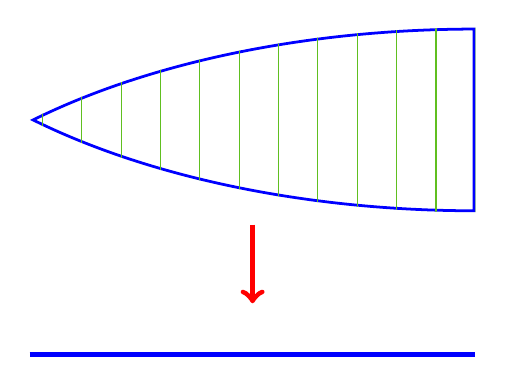
\begin{tikzpicture}[baseline=-0.15cm]
\begin{scope}
\path[clip] (0,1) arc (90:135:8 and 4)  arc (-135:-90:8 and 4) -- cycle;
\draw[blue,line width=2pt] (0,1) arc (90:135:8 and 4)  arc (-135:-90:8 and 4) -- cycle;
\foreach \x in {-6, -5.5, ..., 0} {
	\draw[green!50!brown] (\x,-2) -- (\x,2);
}
\end{scope}
\draw[blue,line width=1.5pt] (-5.66,-3.15) -- (0,-3.15);
\draw[->,red,line width=2pt] (-2.83,-1.5) -- (-2.83,-2.5);
\end{tikzpicture}
$$
\caption{Examples of pinched products}\label{pinched_prods}
\end{figure}
(The need for a strengthened version will become apparent in Appendix \ref{sec:comparing-defs}
where we construct a traditional category from a topological category.)
Define a {\it pinched product} to be a map
\[
	\pi: E\to X
\]
such that $E$ is a $k{+}m$-ball, $X$ is a $k$-ball ($m\ge 1$), and $\pi$ is locally modeled
on a standard iterated degeneracy map
\[
	d: \Delta^{k+m}\to\Delta^k .
\]
(We thank Kevin Costello for suggesting this approach.)

Note that for each interior point $x\in X$, $\pi\inv(x)$ is an $m$-ball,
and for for each boundary point $x\in\bd X$, $\pi\inv(x)$ is a ball of dimension
$l \le m$, with $l$ depending on $x$.

It is easy to see that a composition of pinched products is again a pinched product.

A {\it sub pinched product} is a sub-$m$-ball $E'\sub E$ such that the restriction
$\pi:E'\to \pi(E')$ is again a pinched product.
A {union} of pinched products is a decomposition $E = \cup_i E_i$
such that each $E_i\sub E$ is a sub pinched product.
(See Figure \ref{pinched_prod_unions}.)
\begin{figure}[t]
$$
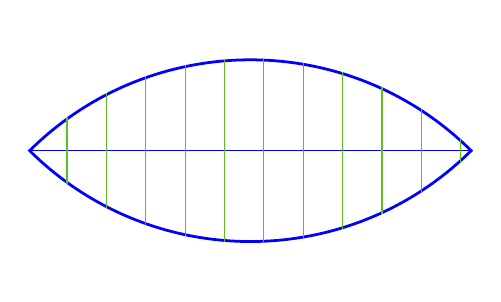
\begin{tikzpicture}[baseline=0]
\begin{scope}
\path[clip] (0,0) arc (135:45:4) arc (-45:-135:4);
\draw[blue,line width=2pt] (0,0) arc (135:45:4) arc (-45:-135:4);
\draw[blue] (0,0) -- (5.66,0);
\foreach \x in {0, 0.5, ..., 6} {
	\draw[green!50!brown] (\x,-2) -- (\x,2);
}
\end{scope}
\end{tikzpicture}
\qquad
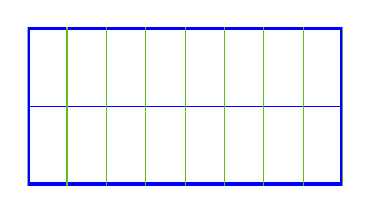
\begin{tikzpicture}[baseline=0]
\begin{scope}
\path[clip] (0,-1) rectangle (4,1);
\draw[blue,line width=2pt] (0,-1) rectangle (4,1);
\draw[blue] (0,0) -- (5,0);
\foreach \x in {0, 0.5, ..., 6} {
	\draw[green!50!brown] (\x,-2) -- (\x,2);
}
\end{scope}
\end{tikzpicture}
\qquad
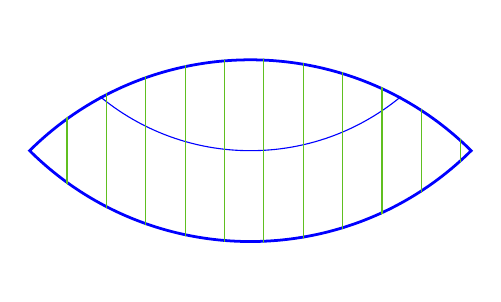
\begin{tikzpicture}[baseline=0]
\begin{scope}
\path[clip] (0,0) arc (135:45:4) arc (-45:-135:4);
\draw[blue,line width=2pt] (0,0) arc (135:45:4) arc (-45:-135:4);
\draw[blue] (2.83,3) circle (3);
\foreach \x in {0, 0.5, ..., 6} {
	\draw[green!50!brown] (\x,-2) -- (\x,2);
}
\end{scope}
\end{tikzpicture}
$$
$$
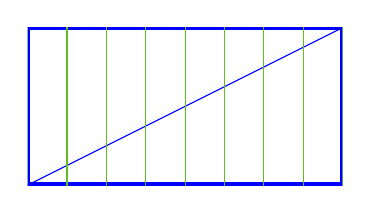
\begin{tikzpicture}[baseline=0]
\begin{scope}
\path[clip] (0,-1) rectangle (4,1);
\draw[blue,line width=2pt] (0,-1) rectangle (4,1);
\draw[blue] (0,-1) -- (4,1);
\foreach \x in {0, 0.5, ..., 6} {
	\draw[green!50!brown] (\x,-2) -- (\x,2);
}
\end{scope}
\end{tikzpicture}
\qquad
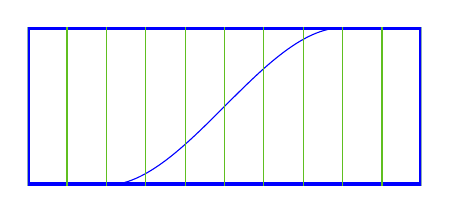
\begin{tikzpicture}[baseline=0]
\begin{scope}
\path[clip] (0,-1) rectangle (5,1);
\draw[blue,line width=2pt] (0,-1) rectangle (5,1);
\draw[blue] (1,-1) .. controls  (2,-1) and (3,1) .. (4,1);
\foreach \x in {0, 0.5, ..., 6} {
	\draw[green!50!brown] (\x,-2) -- (\x,2);
}
\end{scope}
\end{tikzpicture}
$$
\caption{Five examples of unions of pinched products}\label{pinched_prod_unions}
\end{figure}

The product axiom will give a map $\pi^*:\cC(X)\to \cC(E)$ for each pinched product
$\pi:E\to X$.
Morphisms in the image of $\pi^*$ will be called product morphisms.
Before stating the axiom, we illustrate it in our two motivating examples of $n$-categories.
In the case where $\cC(X) = \{f: X\to T\}$, we define $\pi^*(f) = f\circ\pi$.
In the case where $\cC(X)$ is the set of all labeled embedded cell complexes $K$ in $X$, 
define $\pi^*(K) = \pi\inv(K)$, with each codimension $i$ cell $\pi\inv(c)$ labeled by the
same (traditional) $i$-morphism as the corresponding codimension $i$ cell $c$.


\addtocounter{axiom}{-1}
\begin{axiom}[Product (identity) morphisms]
For each pinched product $\pi:E\to X$, with $X$ a $k$-ball and $E$ a $k{+}m$-ball ($m\ge 1$),
there is a map $\pi^*:\cC(X)\to \cC(E)$.
These maps must satisfy the following conditions.
\begin{enumerate}
\item
If $\pi:E\to X$ and $\pi':E'\to X'$ are pinched products, and
if $f:X\to X'$ and $\tilde{f}:E \to E'$ are maps such that the diagram
\[ \xymatrix{
	E \ar[r]^{\tilde{f}} \ar[d]_{\pi} & E' \ar[d]^{\pi'} \\
	X \ar[r]^{f} & X'
} \]
commutes, then we have 
\[
	\pi'^*\circ f = \tilde{f}\circ \pi^*.
\]
\item
Product morphisms are compatible with gluing (composition).
Let $\pi:E\to X$, $\pi_1:E_1\to X_1$, and $\pi_2:E_2\to X_2$ 
be pinched products with $E = E_1\cup E_2$.
Let $a\in \cC(X)$, and let $a_i$ denote the restriction of $a$ to $X_i\sub X$.
Then 
\[
	\pi^*(a) = \pi_1^*(a_1)\bullet \pi_2^*(a_2) .
\]
\item
Product morphisms are associative.
If $\pi:E\to X$ and $\rho:D\to E$ are pinched products then
\[
	\rho^*\circ\pi^* = (\pi\circ\rho)^* .
\]
\item
Product morphisms are compatible with restriction.
If we have a commutative diagram
\[ \xymatrix{
	D \ar@{^(->}[r] \ar[d]_{\rho} & E \ar[d]^{\pi} \\
	Y \ar@{^(->}[r] & X
} \]
such that $\rho$ and $\pi$ are pinched products, then
\[
	\res_D\circ\pi^* = \rho^*\circ\res_Y .
\]
\end{enumerate}
\end{axiom}


\medskip

All of the axioms listed above hold for both ordinary $n$-categories and $A_\infty$ $n$-categories.
The last axiom (below), concerning actions of 
homeomorphisms in the top dimension $n$, distinguishes the two cases.

We start with the plain $n$-category case.

\begin{axiom}[\textup{\textbf{[preliminary]}} Isotopy invariance in dimension $n$]
Let $X$ be an $n$-ball and $f: X\to X$ be a homeomorphism which restricts
to the identity on $\bd X$ and is isotopic (rel boundary) to the identity.
Then $f$ acts trivially on $\cC(X)$; $f(a) = a$ for all $a\in \cC(X)$.
\end{axiom}

This axiom needs to be strengthened to force product morphisms to act as the identity.
Let $X$ be an $n$-ball and $Y\sub\bd X$ be an $n{-}1$-ball.
Let $J$ be a 1-ball (interval).
We have a collaring homeomorphism $s_{Y,J}: X\cup_Y (Y\times J) \to X$.
(Here we use the ``pinched" version of $Y\times J$.
\nn{do we need notation for this?})
We define a map
\begin{eqnarray*}
	\psi_{Y,J}: \cC(X) &\to& \cC(X) \\
	a & \mapsto & s_{Y,J}(a \cup ((a|_Y)\times J)) .
\end{eqnarray*}
(See Figure \ref{glue-collar}.)
\begin{figure}[!ht]
\begin{equation*}
\begin{tikzpicture}
\def\rad{1}
\def\srad{0.75}
\def\gap{4.5}
\foreach \i in {0, 1, 2} {
	\node(\i) at ($\i*(\gap,0)$) [draw, circle through = {($\i*(\gap,0)+(\rad,0)$)}] {};
	\node(\i-small) at (\i.east) [circle through={($(\i.east)+(\srad,0)$)}] {};
	\foreach \n in {1,2} {
		\fill (intersection \n of \i-small and \i) node(\i-intersection-\n) {} circle (2pt);
	}
}

\begin{scope}[decoration={brace,amplitude=10,aspect=0.5}]
	\draw[decorate] (0-intersection-1.east) -- (0-intersection-2.east);
\end{scope}
\node[right=1mm] at (0.east) {$a$};
\draw[->] ($(0.east)+(0.75,0)$) -- ($(1.west)+(-0.2,0)$);

\draw (1-small)  circle (\srad);
\foreach \theta in {90, 72, ..., -90} {
	\draw[blue] (1) -- ($(1)+(\rad,0)+(\theta:\srad)$);
}
\filldraw[fill=white] (1) circle (\rad);
\foreach \n in {1,2} {
	\fill (intersection \n of 1-small and 1) circle (2pt);
}
\node[below] at (1-small.south) {$a \times J$};
\draw[->] ($(1.east)+(1,0)$) -- ($(2.west)+(-0.2,0)$);

\begin{scope}
\path[clip] (2) circle (\rad);
\draw[clip] (2.east) circle (\srad);
\foreach \y in {1, 0.86, ..., -1} {
	\draw[blue] ($(2)+(-1,\y) $)-- ($(2)+(1,\y)$);
}
\end{scope}
\end{tikzpicture}
\end{equation*}
\begin{equation*}
\xymatrix@C+2cm{\cC(X) \ar[r]^(0.45){\text{glue}} & \cC(X \cup \text{collar}) \ar[r]^(0.55){\text{homeo}} & \cC(X)}
\end{equation*}

\caption{Extended homeomorphism.}\label{glue-collar}\end{figure}
We call a map of this form a {\it collar map}.
It can be thought of as the action of the inverse of
a map which projects a collar neighborhood of $Y$ onto $Y$,
or as the limit of homeomorphisms $X\to X$ which expand a very thin collar of $Y$
to a larger collar.
We call the equivalence relation generated by collar maps and homeomorphisms
isotopic (rel boundary) to the identity {\it extended isotopy}.

The revised axiom is

\addtocounter{axiom}{-1}
\begin{axiom}[\textup{\textbf{[plain  version]}} Extended isotopy invariance in dimension $n$.]
\label{axiom:extended-isotopies}
Let $X$ be an $n$-ball and $f: X\to X$ be a homeomorphism which restricts
to the identity on $\bd X$ and isotopic (rel boundary) to the identity.
Then $f$ acts trivially on $\cC(X)$.
In addition, collar maps act trivially on $\cC(X)$.
\end{axiom}

\smallskip

For $A_\infty$ $n$-categories, we replace
isotopy invariance with the requirement that families of homeomorphisms act.
For the moment, assume that our $n$-morphisms are enriched over chain complexes.
Let $\Homeo_\bd(X)$ denote homeomorphisms of $X$ which fix $\bd X$ and
$C_*(\Homeo_\bd(X))$ denote the singular chains on this space.


\addtocounter{axiom}{-1}
\begin{axiom}[\textup{\textbf{[$A_\infty$ version]}} Families of homeomorphisms act in dimension $n$.]
For each $n$-ball $X$ and each $c\in \cl{\cC}(\bd X)$ we have a map of chain complexes
\[
	C_*(\Homeo_\bd(X))\ot \cC(X; c) \to \cC(X; c) .
\]
These action maps are required to be associative up to homotopy,
%\nn{iterated homotopy?}
and also compatible with composition (gluing) in the sense that
a diagram like the one in Theorem \ref{thm:CH} commutes.
%\nn{repeat diagram here?}
%\nn{restate this with $\Homeo(X\to X')$?  what about boundary fixing property?}
\end{axiom}

We should strengthen the above axiom to apply to families of collar maps.
To do this we need to explain how collar maps form a topological space.
Roughly, the set of collared $n{-}1$-balls in the boundary of an $n$-ball has a natural topology,
and we can replace the class of all intervals $J$ with intervals contained in $\r$.
Having chains on the space of collar maps act gives rise to coherence maps involving
weak identities.
We will not pursue this in detail here.

Note that if we take homology of chain complexes, we turn an $A_\infty$ $n$-category
into a plain $n$-category (enriched over graded groups).
In a different direction, if we enrich over topological spaces instead of chain complexes,
we get a space version of an $A_\infty$ $n$-category, with $\Homeo_\bd(X)$ acting 
instead of  $C_*(\Homeo_\bd(X))$.
Taking singular chains converts such a space type $A_\infty$ $n$-category into a chain complex
type $A_\infty$ $n$-category.

\medskip

The alert reader will have already noticed that our definition of a (plain) $n$-category
is extremely similar to our definition of a system of fields.
There are two differences.
First, for the $n$-category definition we restrict our attention to balls
(and their boundaries), while for fields we consider all manifolds.
Second,  in category definition we directly impose isotopy
invariance in dimension $n$, while in the fields definition we 
instead remember a subspace of local relations which contain differences of isotopic fields. 
(Recall that the compensation for this complication is that we can demand that the gluing map for fields is injective.)
Thus a system of fields and local relations $(\cF,\cU)$ determines an $n$-category $\cC_ {\cF,\cU}$ simply by restricting our attention to
balls and, at level $n$, quotienting out by the local relations:
\begin{align*}
\cC_{\cF,\cU}(B^k) & = \begin{cases}\cF(B) & \text{when $k<n$,} \\ \cF(B) / \cU(B) & \text{when $k=n$.}\end{cases}
\end{align*}
This $n$-category can be thought of as the local part of the fields.
Conversely, given a topological $n$-category we can construct a system of fields via 
a colimit construction; see \S \ref{ss:ncat_fields} below.

\subsection{Examples of $n$-categories}
\label{ss:ncat-examples}


We now describe several classes of examples of $n$-categories satisfying our axioms.
We typically specify only the morphisms; the rest of the data for the category
(restriction maps, gluing, product morphisms, action of homeomorphisms) is usually obvious.

\begin{example}[Maps to a space]
\rm
\label{ex:maps-to-a-space}%
Let $T$ be a topological space.
We define $\pi_{\leq n}(T)$, the fundamental $n$-category of $T$, as follows.
For $X$ a $k$-ball with $k < n$, define $\pi_{\leq n}(T)(X)$ to be the set of 
all continuous maps from $X$ to $T$.
For $X$ an $n$-ball define $\pi_{\leq n}(T)(X)$ to be continuous maps from $X$ to $T$ modulo
homotopies fixed on $\bd X$.
(Note that homotopy invariance implies isotopy invariance.)
For $a\in \cC(X)$ define the product morphism $a\times D \in \cC(X\times D)$ to
be $a\circ\pi_X$, where $\pi_X : X\times D \to X$ is the projection.
\end{example}

\noop{
Recall we described a system of fields and local relations based on maps to $T$ in Example \ref{ex:maps-to-a-space(fields)} above.
Constructing a system of fields from $\pi_{\leq n}(T)$ recovers that example.
\nn{shouldn't this go elsewhere?  we haven't yet discussed constructing a system of fields from
an n-cat}
}

\begin{example}[Maps to a space, with a fiber] \label{ex:maps-with-fiber}
\rm
\label{ex:maps-to-a-space-with-a-fiber}%
We can modify the example above, by fixing a
closed $m$-manifold $F$, and defining $\pi^{\times F}_{\leq n}(T)(X) = \Maps(X \times F \to T)$, 
otherwise leaving the definition in Example \ref{ex:maps-to-a-space} unchanged.
Taking $F$ to be a point recovers the previous case.
\end{example}

\begin{example}[Linearized, twisted, maps to a space]
\rm
\label{ex:linearized-maps-to-a-space}%
We can linearize Examples \ref{ex:maps-to-a-space} and \ref{ex:maps-to-a-space-with-a-fiber} as follows.
Let $\alpha$ be an $(n{+}m{+}1)$-cocycle on $T$ with values in a ring $R$
(have in mind the trivial cocycle).
For $X$ of dimension less than $n$ define $\pi^{\alpha, \times F}_{\leq n}(T)(X)$ as before, ignoring $\alpha$.
For $X$ an $n$-ball and $c\in \Maps(\bdy X \times F \to T)$ define $\pi^{\alpha, \times F}_{\leq n}(T)(X; c)$ to be
the $R$-module of finite linear combinations of continuous maps from $X\times F$ to $T$,
modulo the relation that if $a$ is homotopic to $b$ (rel boundary) via a homotopy
$h: X\times F\times I \to T$, then $a = \alpha(h)b$.
(In order for this to be well-defined we must choose $\alpha$ to be zero on degenerate simplices.
Alternatively, we could equip the balls with fundamental classes.)
\end{example}

\begin{example}[$n$-categories from TQFTs]
\rm
\label{ex:ncats-from-tqfts}%
Let $\cF$ be a TQFT in the sense of \S\ref{sec:fields}: an $n$-dimensional 
system of fields (also denoted $\cF$) and local relations.
Let $W$ be an $n{-}j$-manifold.
Define the $j$-category $\cF(W)$ as follows.
If $X$ is a $k$-ball with $k<j$, let $\cF(W)(X) \deq \cF(W\times X)$.
If $X$ is a $j$-ball and $c\in \cl{\cF(W)}(\bd X)$, 
let $\cF(W)(X; c) \deq A_\cF(W\times X; c)$.
\end{example}

The next example is only intended to be illustrative, as we don't specify 
which definition of a ``traditional $n$-category" we intend.
Further, most of these definitions don't even have an agreed-upon notion of 
``strong duality", which we assume here.
\begin{example}[Traditional $n$-categories]
\rm
\label{ex:traditional-n-categories}
Given a ``traditional $n$-category with strong duality" $C$
define $\cC(X)$, for $X$ a $k$-ball with $k < n$,
to be the set of all $C$-labeled embedded cell complexes of $X$ (c.f. \S \ref{sec:fields}).
For $X$ an $n$-ball and $c\in \cl{\cC}(\bd X)$, define $\cC(X; c)$ to be finite linear
combinations of $C$-labeled embedded cell complexes of $X$
modulo the kernel of the evaluation map.
Define a product morphism $a\times D$, for $D$ an $m$-ball, to be the product of the cell complex of $a$ with $D$,
with each cell labelled according to the corresponding cell for $a$.
(These two cells have the same codimension.)
More generally, start with an $n{+}m$-category $C$ and a closed $m$-manifold $F$.
Define $\cC(X)$, for $\dim(X) < n$,
to be the set of all $C$-labeled embedded cell complexes of $X\times F$.
Define $\cC(X; c)$, for $X$ an $n$-ball,
to be the dual Hilbert space $A(X\times F; c)$.
(See \S\ref{sec:constructing-a-tqft}.)
\end{example}

\noop{
\nn{shouldn't this go elsewhere?  we haven't yet discussed constructing a system of fields from
an n-cat}
Recall we described a system of fields and local relations based on a ``traditional $n$-category" 
$C$ in Example \ref{ex:traditional-n-categories(fields)} above.
\nn{KW: We already refer to \S \ref{sec:fields} above}
Constructing a system of fields from $\cC$ recovers that example. 
\todo{Except that it doesn't: pasting diagrams v.s. string diagrams.}
\nn{KW: but the above example is all about string diagrams.  the only difference is at the top level,
where the quotient is built in.
but (string diagrams)/(relations) is isomorphic to 
(pasting diagrams composed of smaller string diagrams)/(relations)}
}


\newcommand{\Bord}{\operatorname{Bord}}
\begin{example}[The bordism $n$-category, plain version]
\label{ex:bord-cat}
\rm
\label{ex:bordism-category}
For a $k$-ball $X$, $k<n$, define $\Bord^n(X)$ to be the set of all $k$-dimensional
submanifolds $W$ of $X\times \Real^\infty$ such that the projection $W \to X$ is transverse
to $\bd X$.
For an $n$-ball $X$ define $\Bord^n(X)$ to be homeomorphism classes (rel boundary) of such $n$-dimensional submanifolds;
we identify $W$ and $W'$ if $\bd W = \bd W'$ and there is a homeomorphism
$W \to W'$ which restricts to the identity on the boundary.
\end{example}

%\nn{the next example might be an unnecessary distraction.  consider deleting it.}

%\begin{example}[Variation on the above examples]
%We could allow $F$ to have boundary and specify boundary conditions on $X\times \bd F$,
%for example product boundary conditions or take the union over all boundary conditions.
%%\nn{maybe should not emphasize this case, since it's ``better" in some sense
%%to think of these guys as affording a representation
%%of the $n{+}1$-category associated to $\bd F$.}
%\end{example}


%We have two main examples of $A_\infty$ $n$-categories, coming from maps to a target space and from the blob complex.

\begin{example}[Chains (or space) of maps to a space]
\rm
\label{ex:chains-of-maps-to-a-space}
We can modify Example \ref{ex:maps-to-a-space} above to define the fundamental $A_\infty$ $n$-category $\pi^\infty_{\le n}(T)$ of a topological space $T$.
For a $k$-ball $X$, with $k < n$, the set $\pi^\infty_{\leq n}(T)(X)$ is just $\Maps(X \to T)$.
Define $\pi^\infty_{\leq n}(T)(X; c)$ for an $n$-ball $X$ and $c \in \pi^\infty_{\leq n}(T)(\bdy X)$ to be the chain complex
\[
	C_*(\Maps_c(X\times F \to T)),
\]
where $\Maps_c$ denotes continuous maps restricting to $c$ on the boundary,
and $C_*$ denotes singular chains.
Alternatively, if we take the $n$-morphisms to be simply $\Maps_c(X\times F \to T)$, 
we get an $A_\infty$ $n$-category enriched over spaces.
\end{example}

See also Theorem \ref{thm:map-recon} below, recovering $C_*(\Maps(M \to T))$ up to 
homotopy the blob complex of $M$ with coefficients in $\pi^\infty_{\le n}(T)$.

\begin{example}[Blob complexes of balls (with a fiber)]
\rm
\label{ex:blob-complexes-of-balls}
Fix an $n{-}k$-dimensional manifold $F$ and an $n$-dimensional system of fields $\cE$.
We will define an $A_\infty$ $k$-category $\cC$.
When $X$ is a $m$-ball, with $m<k$, define $\cC(X) = \cE(X\times F)$.
When $X$ is an $k$-ball,
define $\cC(X; c) = \bc^\cE_*(X\times F; c)$
where $\bc^\cE_*$ denotes the blob complex based on $\cE$.
\end{example}

This example will be used in Theorem \ref{thm:product} below, which allows us to compute the blob complex of a product.
Notice that with $F$ a point, the above example is a construction turning a topological 
$n$-category $\cC$ into an $A_\infty$ $n$-category.
We think of this as providing a ``free resolution" 
of the topological $n$-category. 
%\nn{say something about cofibrant replacements?}
In fact, there is also a trivial, but mostly uninteresting, way to do this: 
we can think of each vector space associated to an $n$-ball as a chain complex concentrated in degree $0$, 
and take $\CD{B}$ to act trivially. 

Be careful that the ``free resolution" of the topological $n$-category $\pi_{\leq n}(T)$ is not the $A_\infty$ $n$-category $\pi^\infty_{\leq n}(T)$.
It's easy to see that with $n=0$, the corresponding system of fields is just 
linear combinations of connected components of $T$, and the local relations are trivial.
There's no way for the blob complex to magically recover all the data of $\pi^\infty_{\leq 0}(T) \iso C_* T$.

\begin{example}[The bordism $n$-category, $A_\infty$ version]
\rm
\label{ex:bordism-category-ainf}
As in Example \ref{ex:bord-cat}, for $X$ a $k$-ball, $k<n$, we define $\Bord^{n,\infty}(X)$
to be the set of all $k$-dimensional
submanifolds $W$ of $X\times \Real^\infty$ such that the projection $W \to X$ is transverse
to $\bd X$.
For an $n$-ball $X$ with boundary condition $c$ 
define $\Bord^{n,\infty}(X; c)$ to be the space of all $k$-dimensional
submanifolds $W$ of $X\times \Real^\infty$ such that 
$W$ coincides with $c$ at $\bd X \times \Real^\infty$.
(The topology on this space is induced by ambient isotopy rel boundary.
This is homotopy equivalent to a disjoint union of copies $\mathrm{B}\!\Homeo(W')$, where
$W'$ runs though representatives of homeomorphism types of such manifolds.)
\end{example}



Let $\cE\cB_n$ be the operad of smooth embeddings of $k$ (little)
copies of the standard $n$-ball $B^n$ into another (big) copy of $B^n$.
(We require that the interiors of the little balls be disjoint, but their 
boundaries are allowed to meet.
Note in particular that the space for $k=1$ contains a copy of $\Diff(B^n)$, namely
the embeddings of a ``little" ball with image all of the big ball $B^n$.
(But note also that this inclusion is not
necessarily a homotopy equivalence.)
The operad $\cE\cB_n$ is homotopy equivalent to the standard framed little $n$-ball operad:
by shrinking the little balls (precomposing them with dilations), 
we see that both operads are homotopic to the space of $k$ framed points
in $B^n$.
It is easy to see that $n$-fold loop spaces $\Omega^n(T)$  have
an action of $\cE\cB_n$.
%\nn{add citation for this operad if we can find one}

\begin{example}[$E_n$ algebras]
\rm
\label{ex:e-n-alg}

Let $A$ be an $\cE\cB_n$-algebra.
Note that this implies a $\Diff(B^n)$ action on $A$, 
since $\cE\cB_n$ contains a copy of $\Diff(B^n)$.
We will define an $A_\infty$ $n$-category $\cC^A$.
If $X$ is a ball of dimension $k<n$, define $\cC^A(X)$ to be a point.
In other words, the $k$-morphisms are trivial for $k<n$.
If $X$ is an $n$-ball, we define $\cC^A(X)$ via a colimit construction.
(Plain colimit, not homotopy colimit.)
Let $J$ be the category whose objects are embeddings of a disjoint union of copies of 
the standard ball $B^n$ into $X$, and who morphisms are given by engulfing some of the 
embedded balls into a single larger embedded ball.
To each object of $J$ we associate $A^{\times m}$ (where $m$ is the number of balls), and
to each morphism of $J$ we associate a morphism coming from the $\cE\cB_n$ action on $A$.
Alternatively and more simply, we could define $\cC^A(X)$ to be 
$\Diff(B^n\to X)\times A$ modulo the diagonal action of $\Diff(B^n)$.
The remaining data for the $A_\infty$ $n$-category 
--- composition and $\Diff(X\to X')$ action ---
also comes from the $\cE\cB_n$ action on $A$.
\nn{should we spell this out?}

\nn{Should remark that the associated hocolim for manifolds
agrees with Lurie's topological chiral homology construction; maybe wait
until next subsection to say that?}

Conversely, one can show that a topological $A_\infty$ $n$-category $\cC$, where the $k$-morphisms
$\cC(X)$ are trivial (single point) for $k<n$, gives rise to 
an $\cE\cB_n$-algebra.
\nn{The paper is already long; is it worth giving details here?}
\end{example}


\subsection{From balls to manifolds}
\label{ss:ncat_fields} \label{ss:ncat-coend}
In this section we describe how to extend an $n$-category $\cC$ as described above 
(of either the plain or $A_\infty$ variety) to an invariant of manifolds, which we denote by $\cl{\cC}$.
This extension is a certain colimit, and we've chosen the notation to remind you of this.
Thus we show that functors $\cC_k$ satisfying the axioms above have a canonical extension 
from $k$-balls to arbitrary $k$-manifolds.
Recall that we've already anticipated this construction in the previous section, 
inductively defining $\cl{\cC}$ on $k$-spheres in terms of $\cC$ on $k$-balls, 
so that we can state the boundary axiom for $\cC$ on $k+1$-balls.
In the case of plain $n$-categories, this construction factors into a construction of a 
system of fields and local relations, followed by the usual TQFT definition of a 
vector space invariant of manifolds given as Definition \ref{defn:TQFT-invariant}.
For an $A_\infty$ $n$-category, $\cl{\cC}$ is defined using a homotopy colimit instead.
Recall that we can take a plain $n$-category $\cC$ and pass to the ``free resolution", 
an $A_\infty$ $n$-category $\bc_*(\cC)$, by computing the blob complex of balls 
(recall Example \ref{ex:blob-complexes-of-balls} above).
We will show in Corollary \ref{cor:new-old} below that the homotopy colimit invariant 
for a manifold $M$ associated to this $A_\infty$ $n$-category is actually the 
same as the original blob complex  for $M$ with coefficients in $\cC$.

We will first define the ``decomposition" poset $\cell(W)$ for any $k$-manifold $W$, for $1 \leq k \leq n$. 
An $n$-category $\cC$ provides a functor from this poset to the category of sets, 
and we  will define $\cl{\cC}(W)$ as a suitable colimit 
(or homotopy colimit in the $A_\infty$ case) of this functor. 
We'll later give a more explicit description of this colimit.
In the case that the $n$-category $\cC$ is enriched (e.g. associates vector spaces or chain complexes to $n$-balls with boundary data), 
then the resulting colimit is also enriched, that is, the set associated to $W$ splits into subsets according to boundary data, and each of these subsets has the appropriate structure (e.g. a vector space or chain complex).

Recall (Definition \ref{defn:gluing-decomposition}) that a {\it ball decomposition} of $W$ is a 
sequence of gluings $M_0\to M_1\to\cdots\to M_m = W$ such that $M_0$ is a disjoint union of balls
$\du_a X_a$.
Abusing notation, we let $X_a$ denote both the ball (component of $M_0$) and
its image in $W$ (which is not necessarily a ball --- parts of $\bd X_a$ may have been glued together).
Define a {\it permissible decomposition} of $W$ to be a map
\[
	\coprod_a X_a \to W,
\]
which can be completed to a ball decomposition $\du_a X_a = M_0\to\cdots\to M_m = W$.
Roughly, a permissible decomposition is like a ball decomposition where we don't care in which order the balls
are glued up to yield $W$, so long as there is some (non-pathological) way to glue them.

Given permissible decompositions $x = \{X_a\}$ and $y = \{Y_b\}$ of $W$, we say that $x$ is a refinement
of $y$, or write $x \le y$, if there is a ball decomposition $\du_a X_a = M_0\to\cdots\to M_m = W$
with $\du_b Y_b = M_i$ for some $i$.

\begin{defn}
The poset $\cell(W)$ has objects the permissible decompositions of $W$, 
and a unique morphism from $x$ to $y$ if and only if $x$ is a refinement of $y$.
See Figure \ref{partofJfig} for an example.
\end{defn}

\begin{figure}[!ht]
\begin{equation*}
\mathfig{.63}{ncat/zz2}
\end{equation*}
\caption{A small part of $\cell(W)$}
\label{partofJfig}
\end{figure}

An $n$-category $\cC$ determines 
a functor $\psi_{\cC;W}$ from $\cell(W)$ to the category of sets 
(possibly with additional structure if $k=n$).
Each $k$-ball $X$ of a decomposition $y$ of $W$ has its boundary decomposed into $k{-}1$-balls,
and, as described above, we have a subset $\cC(X)\spl \sub \cC(X)$ of morphisms whose boundaries
are splittable along this decomposition.

\begin{defn}
Define the functor $\psi_{\cC;W} : \cell(W) \to \Set$ as follows.
For a decomposition $x = \bigcup_a X_a$ in $\cell(W)$, $\psi_{\cC;W}(x)$ is the subset
\begin{equation}
\label{eq:psi-C}
	\psi_{\cC;W}(x) \sub \prod_a \cC(X_a)\spl
\end{equation}
where the restrictions to the various pieces of shared boundaries amongst the cells
$X_a$ all agree (this is a fibered product of all the labels of $n$-cells over the labels of $n-1$-cells).
If $x$ is a refinement of $y$, the map $\psi_{\cC;W}(x) \to \psi_{\cC;W}(y)$ is given by the composition maps of $\cC$.
\end{defn}

If $k=n$ in the above definition and we are enriching in some auxiliary category, 
we need to say a bit more.
We can rewrite Equation \ref{eq:psi-C} as
\begin{equation} \label{eq:psi-CC}
	\psi_{\cC;W}(x) \deq \coprod_\beta \prod_a \cC(X_a; \beta) ,
\end{equation}
where $\beta$ runs through labelings of the $k{-}1$-skeleton of the decomposition
(which are compatible when restricted to the $k{-}2$-skeleton), and $\cC(X_a; \beta)$
means the subset of $\cC(X_a)$ whose restriction to $\bd X_a$ agress with $\beta$.
If we are enriching over $\cS$ and $k=n$, then $\cC(X_a; \beta)$ is an object in 
$\cS$ and the coproduct and product in Equation \ref{eq:psi-CC} should be replaced by the approriate
operations in $\cS$ (e.g. direct sum and tensor product if $\cS$ is Vect).

Finally, we construct $\cl{\cC}(W)$ as the appropriate colimit of $\psi_{\cC;W}$.

\begin{defn}[System of fields functor]
\label{def:colim-fields}
If $\cC$ is an $n$-category enriched in sets or vector spaces, $\cl{\cC}(W)$ is the usual colimit of the functor $\psi_{\cC;W}$.
That is, for each decomposition $x$ there is a map
$\psi_{\cC;W}(x)\to \cl{\cC}(W)$, these maps are compatible with the refinement maps
above, and $\cl{\cC}(W)$ is universal with respect to these properties.
\end{defn}

\begin{defn}[System of fields functor, $A_\infty$ case]
When $\cC$ is an $A_\infty$ $n$-category, $\cl{\cC}(W)$ for $W$ a $k$-manifold with $k < n$ 
is defined as above, as the colimit of $\psi_{\cC;W}$.
When $W$ is an $n$-manifold, the chain complex $\cl{\cC}(W)$ is the homotopy colimit of the functor $\psi_{\cC;W}$.
\end{defn}

We can specify boundary data $c \in \cl{\cC}(\bdy W)$, and define functors $\psi_{\cC;W,c}$ 
with values the subsets of those of $\psi_{\cC;W}$ which agree with $c$ on the boundary of $W$.

We now give more concrete descriptions of the above colimits.

In the non-enriched case (e.g.\ $k<n$), where each $\cC(X_a; \beta)$ is just a set,
the colimit is
\[
	\cl{\cC}(W,c) = \left( \coprod_x \coprod_\beta \prod_a \cC(X_a; \beta) \right) / \sim ,
\]
where $x$ runs through decomposition of $W$, and $\sim$ is the obvious equivalence relation 
induced by refinement and gluing.
If $\cC$ is enriched over vector spaces and $W$ is an $n$-manifold, 
we can take
\begin{equation*}
	\cl{\cC}(W,c) = \left( \bigoplus_x \bigoplus_\beta \bigotimes_a \cC(X_a; \beta) \right) / K
\end{equation*}
where $K$ is the vector space spanned by elements $a - g(a)$, with
$a\in \psi_{\cC;W,c}(x)$ for some decomposition $x$, and $g: \psi_{\cC;W,c}(x)
\to \psi_{\cC;W,c}(y)$ is value of $\psi_{\cC;W,c}$ on some antirefinement $x \leq y$.

In the $A_\infty$ case, enriched over chain complexes, the concrete description of the homotopy colimit
is more involved.
Define an $m$-sequence in $W$ to be a sequence $x_0 \le x_1 \le \dots \le x_m$ of permissible decompositions of $W$.
Such sequences (for all $m$) form a simplicial set in $\cell(W)$.
Define $\cl{\cC}(W)$ as a vector space via
\[
	\cl{\cC}(W) = \bigoplus_{(x_i)} \psi_{\cC;W}(x_0)[m] ,
\]
where the sum is over all $m$-sequences $(x_i)$ and all $m$, and each summand is degree shifted by $m$. 
Elements of a summand indexed by an $m$-sequence will be call $m$-simplices.
We endow $\cl{\cC}(W)$ with a differential which is the sum of the differential of the $\psi_{\cC;W}(x_0)$
summands plus another term using the differential of the simplicial set of $m$-sequences.
More specifically, if $(a, \bar{x})$ denotes an element in the $\bar{x}$
summand of $\cl{\cC}(W)$ (with $\bar{x} = (x_0,\dots,x_k)$), define
\[
	\bd (a, \bar{x}) = (\bd a, \bar{x}) + (-1)^{\deg{a}} (g(a), d_0(\bar{x})) + (-1)^{\deg{a}} \sum_{j=1}^k (-1)^{j} (a, d_j(\bar{x})) ,
\]
where $d_j(\bar{x}) = (x_0,\dots,x_{j-1},x_{j+1},\dots,x_k)$ and $g: \psi_\cC(x_0)\to \psi_\cC(x_1)$
is the usual gluing map coming from the antirefinement $x_0 \le x_1$.
%\nn{need to say this better}
%\nn{maybe mention that there is a version that emphasizes minimal gluings (antirefinements) which
%combine only two balls at a time; for $n=1$ this version will lead to usual definition
%of $A_\infty$ category}

We can think of this construction as starting with a disjoint copy of a complex for each
permissible decomposition (the 0-simplices).
Then we glue these together with mapping cylinders coming from gluing maps
(the 1-simplices).
Then we kill the extra homology we just introduced with mapping 
cylinders between the mapping cylinders (the 2-simplices), and so on.

$\cl{\cC}(W)$ is functorial with respect to homeomorphisms of $k$-manifolds. Restricting the $k$-spheres, we have now proved Lemma \ref{lem:spheres}.

It is easy to see that
there are well-defined maps $\cl{\cC}(W)\to\cl{\cC}(\bd W)$, and that these maps
comprise a natural transformation of functors.

\begin{lem}
\label{lem:colim-injective}
Let $W$ be a manifold of dimension less than $n$.  Then for each
decomposition $x$ of $W$ the natural map $\psi_{\cC;W}(x)\to \cl{\cC}(W)$ is injective.
\end{lem}
\begin{proof}
\nn{...}
\end{proof}

\nn{need to finish explaining why we have a system of fields;
define $k$-cat $\cC(\cdot\times W)$}

\subsection{Modules}

Next we define plain and $A_\infty$ $n$-category modules.
The definition will be very similar to that of $n$-categories,
but with $k$-balls replaced by {\it marked $k$-balls,} defined below.

Our motivating example comes from an $(m{-}n{+}1)$-dimensional manifold $W$ with boundary
in the context of an $m{+}1$-dimensional TQFT.
Such a $W$ gives rise to a module for the $n$-category associated to $\bd W$.
This will be explained in more detail as we present the axioms.

Throughout, we fix an $n$-category $\cC$.
For all but one axiom, it doesn't matter whether $\cC$ is a topological $n$-category or an $A_\infty$ $n$-category.
We state the final axiom, on actions of homeomorphisms, differently in the two cases.

Define a {\it marked $k$-ball} to be a pair $(B, N)$ homeomorphic to the pair
$$(\text{standard $k$-ball}, \text{northern hemisphere in boundary of standard $k$-ball}).$$
We call $B$ the ball and $N$ the marking.
A homeomorphism between marked $k$-balls is a homeomorphism of balls which
restricts to a homeomorphism of markings.

\begin{module-axiom}[Module morphisms]
{For each $0 \le k \le n$, we have a functor $\cM_k$ from 
the category of marked $k$-balls and 
homeomorphisms to the category of sets and bijections.}
\end{module-axiom}

(As with $n$-categories, we will usually omit the subscript $k$.)

For example, let $\cD$ be the TQFT which assigns to a $k$-manifold $N$ the set 
of maps from $N$ to $T$ (for $k\le m$), modulo homotopy (and possibly linearized) if $k=m$.
Let $W$ be an $(m{-}n{+}1)$-dimensional manifold with boundary.
Let $\cC$ be the $n$-category with $\cC(X) \deq \cD(X\times \bd W)$.
Let $\cM(B, N) \deq \cD((B\times \bd W)\cup (N\times W))$
(see Example \ref{ex:maps-with-fiber}).
(The union is along $N\times \bd W$.)
%(If $\cD$ were a general TQFT, we would define $\cM(B, N)$ to be
%the subset of $\cD((B\times \bd W)\cup (N\times W))$ which is splittable along $N\times \bd W$.)

\begin{figure}[!ht]
$$\mathfig{.8}{ncat/boundary-collar}$$
\caption{From manifold with boundary collar to marked ball}\label{blah15}\end{figure}

Define the boundary of a marked $k$-ball $(B, N)$ to be the pair $(\bd B \setmin N, \bd N)$.
Call such a thing a {marked $k{-}1$-hemisphere}.

\begin{lem}
\label{lem:hemispheres}
{For each $0 \le k \le n-1$, we have a functor $\cl\cM_k$ from 
the category of marked $k$-hemispheres and 
homeomorphisms to the category of sets and bijections.}
\end{lem}
The proof is exactly analogous to that of Lemma \ref{lem:spheres}, and we omit the details.
We use the same type of colimit construction.

In our example, $\cl\cM(H) = \cD(H\times\bd W \cup \bd H\times W)$.

\begin{module-axiom}[Module boundaries (maps)]
{For each marked $k$-ball $M$ we have a map of sets $\bd: \cM(M)\to \cl\cM(\bd M)$.
These maps, for various $M$, comprise a natural transformation of functors.}
\end{module-axiom}

Given $c\in\cl\cM(\bd M)$, let $\cM(M; c) \deq \bd^{-1}(c)$.

If the $n$-category $\cC$ is enriched over some other category (e.g.\ vector spaces),
then $\cM(M; c)$ should be an object in that category for each marked $n$-ball $M$
and $c\in \cC(\bd M)$.

\begin{lem}[Boundary from domain and range]
{Let $H = M_1 \cup_E M_2$, where $H$ is a marked $k{-}1$-hemisphere ($1\le k\le n$),
$M_i$ is a marked $k{-}1$-ball, and $E = M_1\cap M_2$ is a marked $k{-}2$-hemisphere.
Let $\cM(M_1) \times_{\cM(E)} \cM(M_2)$ denote the fibered product of the 
two maps $\bd: \cM(M_i)\to \cl\cM(E)$.
Then we have an injective map
\[
	\gl_E : \cM(M_1) \times_{\cl\cM(E)} \cM(M_2) \hookrightarrow \cl\cM(H)
\]
which is natural with respect to the actions of homeomorphisms.}
\end{lem}
Again, this is in exact analogy with Lemma \ref{lem:domain-and-range}.

Let $\cl\cM(H)_E$ denote the image of $\gl_E$.
We will refer to elements of $\cl\cM(H)_E$ as ``splittable along $E$" or ``transverse to $E$". 

\begin{lem}[Module to category restrictions]
{For each marked $k$-hemisphere $H$ there is a restriction map
$\cl\cM(H)\to \cC(H)$.  
($\cC(H)$ means apply $\cC$ to the underlying $k$-ball of $H$.)
These maps comprise a natural transformation of functors.}
\end{lem}

Note that combining the various boundary and restriction maps above
(for both modules and $n$-categories)
we have for each marked $k$-ball $(B, N)$ and each $k{-}1$-ball $Y\sub \bd B \setmin N$
a natural map from a subset of $\cM(B, N)$ to $\cC(Y)$.
The subset is the subset of morphisms which are appropriately splittable (transverse to the
cutting submanifolds).
This fact will be used below.

In our example, the various restriction and gluing maps above come from
restricting and gluing maps into $T$.

We require two sorts of composition (gluing) for modules, corresponding to two ways
of splitting a marked $k$-ball into two (marked or plain) $k$-balls.
(See Figure \ref{zzz3}.)

\begin{figure}[!ht]
\begin{equation*}
\mathfig{.4}{ncat/zz3}
\end{equation*}
\caption{Module composition (top); $n$-category action (bottom).}
\label{zzz3}
\end{figure}

First, we can compose two module morphisms to get another module morphism.

\begin{module-axiom}[Module composition]
{Let $M = M_1 \cup_Y M_2$, where $M$, $M_1$ and $M_2$ are marked $k$-balls (with $0\le k\le n$)
and $Y = M_1\cap M_2$ is a marked $k{-}1$-ball.
Let $E = \bd Y$, which is a marked $k{-}2$-hemisphere.
Note that each of $M$, $M_1$ and $M_2$ has its boundary split into two marked $k{-}1$-balls by $E$.
We have restriction (domain or range) maps $\cM(M_i)_E \to \cM(Y)$.
Let $\cM(M_1)_E \times_{\cM(Y)} \cM(M_2)_E$ denote the fibered product of these two maps. 
Then (axiom) we have a map
\[
	\gl_Y : \cM(M_1)_E \times_{\cM(Y)} \cM(M_2)_E \to \cM(M)_E
\]
which is natural with respect to the actions of homeomorphisms, and also compatible with restrictions
to the intersection of the boundaries of $M$ and $M_i$.
If $k < n$ we require that $\gl_Y$ is injective.
(For $k=n$, see below.)}
\end{module-axiom}


Second, we can compose an $n$-category morphism with a module morphism to get another
module morphism.
We'll call this the action map to distinguish it from the other kind of composition.

\begin{module-axiom}[$n$-category action]
{Let $M = X \cup_Y M'$, where $M$ and $M'$ are marked $k$-balls ($0\le k\le n$),
$X$ is a plain $k$-ball,
and $Y = X\cap M'$ is a $k{-}1$-ball.
Let $E = \bd Y$, which is a $k{-}2$-sphere.
We have restriction maps $\cM(M')_E \to \cC(Y)$ and $\cC(X)_E\to \cC(Y)$.
Let $\cC(X)_E \times_{\cC(Y)} \cM(M')_E$ denote the fibered product of these two maps. 
Then (axiom) we have a map
\[
	\gl_Y :\cC(X)_E \times_{\cC(Y)} \cM(M')_E \to \cM(M)_E
\]
which is natural with respect to the actions of homeomorphisms, and also compatible with restrictions
to the intersection of the boundaries of $X$ and $M'$.
If $k < n$ we require that $\gl_Y$ is injective.
(For $k=n$, see below.)}
\end{module-axiom}

\begin{module-axiom}[Strict associativity]
The composition and action maps above are strictly associative.
Given any decomposition of a large marked ball into smaller marked and unmarked balls
any sequence of pairwise gluings yields (via composition and action maps) the same result.
\end{module-axiom}

Note that the above associativity axiom applies to mixtures of module composition,
action maps and $n$-category composition.
See Figure \ref{zzz1b}.

\begin{figure}[!ht]
\begin{equation*}
\mathfig{0.49}{ncat/zz0} \mathfig{0.49}{ncat/zz1}
\end{equation*}
\caption{Two examples of mixed associativity}
\label{zzz1b}
\end{figure}


The above three axioms are equivalent to the following axiom,
which we state in slightly vague form.
\nn{need figure for this}

\xxpar{Module multi-composition:}
{Given any decomposition 
\[
	M =  X_1 \cup\cdots\cup X_p \cup M_1\cup\cdots\cup M_q
\]
of a marked $k$-ball $M$
into small (marked and plain) $k$-balls $M_i$ and $X_j$, there is a 
map from an appropriate subset (like a fibered product) 
of 
\[
	\cC(X_1)\times\cdots\times\cC(X_p) \times \cM(M_1)\times\cdots\times\cM(M_q) 
\]
to $\cM(M)$,
and these various multifold composition maps satisfy an
operad-type strict associativity condition.}

The above operad-like structure is analogous to the swiss cheese operad
\cite{MR1718089}.

\medskip

We can define marked pinched products $\pi:E\to M$ of marked balls analogously to the 
plain ball case.
Note that a marked pinched product can be decomposed into either
two marked pinched products or a plain pinched product and a marked pinched product.
\nn{should give figure}

\begin{module-axiom}[Product (identity) morphisms]
For each pinched product $\pi:E\to M$, with $M$ a marked $k$-ball and $E$ a marked
$k{+}m$-ball ($m\ge 1$),
there is a map $\pi^*:\cM(M)\to \cM(E)$.
These maps must satisfy the following conditions.
\begin{enumerate}
\item
If $\pi:E\to M$ and $\pi':E'\to M'$ are marked pinched products, and
if $f:M\to M'$ and $\tilde{f}:E \to E'$ are maps such that the diagram
\[ \xymatrix{
	E \ar[r]^{\tilde{f}} \ar[d]_{\pi} & E' \ar[d]^{\pi'} \\
	M \ar[r]^{f} & M'
} \]
commutes, then we have 
\[
	\pi'^*\circ f = \tilde{f}\circ \pi^*.
\]
\item
Product morphisms are compatible with module composition and module action.
Let $\pi:E\to M$, $\pi_1:E_1\to M_1$, and $\pi_2:E_2\to M_2$ 
be pinched products with $E = E_1\cup E_2$.
Let $a\in \cM(M)$, and let $a_i$ denote the restriction of $a$ to $M_i\sub M$.
Then 
\[
	\pi^*(a) = \pi_1^*(a_1)\bullet \pi_2^*(a_2) .
\]
Similarly, if $\rho:D\to X$ is a pinched product of plain balls and
$E = D\cup E_1$, then
\[
	\pi^*(a) = \rho^*(a')\bullet \pi_1^*(a_1),
\]
where $a'$ is the restriction of $a$ to $D$.
\item
Product morphisms are associative.
If $\pi:E\to M$ and $\rho:D\to E$ are marked pinched products then
\[
	\rho^*\circ\pi^* = (\pi\circ\rho)^* .
\]
\item
Product morphisms are compatible with restriction.
If we have a commutative diagram
\[ \xymatrix{
	D \ar@{^(->}[r] \ar[d]_{\rho} & E \ar[d]^{\pi} \\
	Y \ar@{^(->}[r] & M
} \]
such that $\rho$ and $\pi$ are pinched products, then
\[
	\res_D\circ\pi^* = \rho^*\circ\res_Y .
\]
($Y$ could be either a marked or plain ball.)
\end{enumerate}
\end{module-axiom}

As in the $n$-category definition, once we have product morphisms we can define
collar maps $\cM(M)\to \cM(M)$.
Note that there are two cases:
the collar could intersect the marking of the marked ball $M$, in which case
we use a product on a morphism of $\cM$; or the collar could be disjoint from the marking,
in which case we use a product on a morphism of $\cC$.

In our example, elements $a$ of $\cM(M)$ maps to $T$, and $\pi^*(a)$ is the pullback of
$a$ along a map associated to $\pi$.

\medskip

There are two alternatives for the next axiom, according whether we are defining
modules for plain $n$-categories or $A_\infty$ $n$-categories.
In the plain case we require

\begin{module-axiom}[\textup{\textbf{[plain version]}} Extended isotopy invariance in dimension $n$]
{Let $M$ be a marked $n$-ball and $f: M\to M$ be a homeomorphism which restricts
to the identity on $\bd M$ and is isotopic (rel boundary) to the identity.
Then $f$ acts trivially on $\cM(M)$.}
In addition, collar maps act trivially on $\cM(M)$.
\end{module-axiom}

We emphasize that the $\bd M$ above means boundary in the marked $k$-ball sense.
In other words, if $M = (B, N)$ then we require only that isotopies are fixed 
on $\bd B \setmin N$.

For $A_\infty$ modules we require

\addtocounter{module-axiom}{-1}
\begin{module-axiom}[\textup{\textbf{[$A_\infty$ version]}} Families of homeomorphisms act]
For each marked $n$-ball $M$ and each $c\in \cM(\bd M)$ we have a map of chain complexes
\[
	C_*(\Homeo_\bd(M))\ot \cM(M; c) \to \cM(M; c) .
\]
Here $C_*$ means singular chains and $\Homeo_\bd(M)$ is the space of homeomorphisms of $M$
which fix $\bd M$.
These action maps are required to be associative up to homotopy, as in Theorem \ref{thm:CH-associativity}, 
and also compatible with composition (gluing) in the sense that
a diagram like the one in Theorem \ref{thm:CH} commutes.
\end{module-axiom}

As with the $n$-category version of the above axiom, we should also have families of collar maps act.

\medskip

Note that the above axioms imply that an $n$-category module has the structure
of an $n{-}1$-category.
More specifically, let $J$ be a marked 1-ball, and define $\cE(X)\deq \cM(X\times J)$,
where $X$ is a $k$-ball and in the product $X\times J$ we pinch 
above the non-marked boundary component of $J$.
(More specifically, we collapse $X\times P$ to a single point, where
$P$ is the non-marked boundary component of $J$.)
Then $\cE$ has the structure of an $n{-}1$-category.

All marked $k$-balls are homeomorphic, unless $k = 1$ and our manifolds
are oriented or Spin (but not unoriented or $\text{Pin}_\pm$).
In this case ($k=1$ and oriented or Spin), there are two types
of marked 1-balls, call them left-marked and right-marked,
and hence there are two types of modules, call them right modules and left modules.
In all other cases ($k>1$ or unoriented or $\text{Pin}_\pm$),
there is no left/right module distinction.

\medskip

We now give some examples of modules over topological and $A_\infty$ $n$-categories.

\begin{example}[Examples from TQFTs]
\rm
Continuing Example \ref{ex:ncats-from-tqfts}, with $\cF$ a TQFT, $W$ an $n{-}j$-manifold,
and $\cF(W)$ the $j$-category associated to $W$.
Let $Y$ be an $(n{-}j{+}1)$-manifold with $\bd Y = W$.
Define a $\cF(W)$ module $\cF(Y)$ as follows.
If $M = (B, N)$ is a marked $k$-ball with $k<j$ let 
$\cF(Y)(M)\deq \cF((B\times W) \cup (N\times Y))$.
If $M = (B, N)$ is a marked $j$-ball and $c\in \cl{\cF(Y)}(\bd M)$ let
$\cF(Y)(M)\deq A_\cF((B\times W) \cup (N\times Y); c)$.
\end{example}

\begin{example}[Examples from the blob complex] \label{bc-module-example}
\rm
In the previous example, we can instead define
$\cF(Y)(M)\deq \bc_*^\cF((B\times W) \cup (N\times Y); c)$ (when $\dim(M) = n$)
and get a module for the $A_\infty$ $n$-category associated to $\cF$ as in 
Example \ref{ex:blob-complexes-of-balls}.
\end{example}


\begin{example}
\rm
Suppose $S$ is a topological space, with a subspace $T$.
We can define a module $\pi_{\leq n}(S,T)$ so that on each marked $k$-ball $(B,N)$ 
for $k<n$ the set $\pi_{\leq n}(S,T)(B,N)$ consists of all continuous maps of pairs 
$(B,N) \to (S,T)$ and on each marked $n$-ball $(B,N)$ it consists of all 
such maps modulo homotopies fixed on $\bdy B \setminus N$.
This is a module over the fundamental $n$-category $\pi_{\leq n}(S)$ of $S$, from Example \ref{ex:maps-to-a-space}.
\end{example}
Modifications corresponding to Examples \ref{ex:maps-to-a-space-with-a-fiber} and 
\ref{ex:linearized-maps-to-a-space} are also possible, and there is an $A_\infty$ version analogous to 
Example \ref{ex:chains-of-maps-to-a-space} given by taking singular chains.

\subsection{Modules as boundary labels (colimits for decorated manifolds)}
\label{moddecss}

Fix a topological $n$-category or $A_\infty$ $n$-category  $\cC$.
Let $W$ be a $k$-manifold ($k\le n$),
let $\{Y_i\}$ be a collection of disjoint codimension 0 submanifolds of $\bd W$,
and let $\cN = (\cN_i)$ be an assignment of a $\cC$ module $\cN_i$ to $Y_i$.

We will define a set $\cC(W, \cN)$ using a colimit construction similar to 
the one appearing in \S \ref{ss:ncat_fields} above.
(If $k = n$ and our $n$-categories are enriched, then
$\cC(W, \cN)$ will have additional structure; see below.)

Define a permissible decomposition of $W$ to be a decomposition
\[
	W = \left(\bigcup_a X_a\right) \cup \left(\bigcup_{i,b} M_{ib}\right) ,
\]
where each $X_a$ is a plain $k$-ball (disjoint from $\cup Y_i$) and
each $M_{ib}$ is a marked $k$-ball intersecting $Y_i$,
with $M_{ib}\cap Y_i$ being the marking.
(See Figure \ref{mblabel}.)
\begin{figure}[t]
\begin{equation*}
\mathfig{.4}{ncat/mblabel}
\end{equation*}
\caption{A permissible decomposition of a manifold
whose boundary components are labeled by $\cC$ modules $\{\cN_i\}$.
Marked balls are shown shaded, plain balls are unshaded.}\label{mblabel}
\end{figure}
Given permissible decompositions $x$ and $y$, we say that $x$ is a refinement
of $y$, or write $x \le y$, if each ball of $y$ is a union of balls of $x$.
This defines a partial ordering $\cell(W)$, which we will think of as a category.
(The objects of $\cell(D)$ are permissible decompositions of $W$, and there is a unique
morphism from $x$ to $y$ if and only if $x$ is a refinement of $y$.)

The collection of modules $\cN$ determines 
a functor $\psi_\cN$ from $\cell(W)$ to the category of sets 
(possibly with additional structure if $k=n$).
For a decomposition $x = (X_a, M_{ib})$ in $\cell(W)$, define $\psi_\cN(x)$ to be the subset
\[
	\psi_\cN(x) \sub \left(\prod_a \cC(X_a)\right) \times \left(\prod_{ib} \cN_i(M_{ib})\right)
\]
such that the restrictions to the various pieces of shared boundaries amongst the
$X_a$ and $M_{ib}$ all agree.
(That is, the fibered product over the boundary restriction maps.)
If $x$ is a refinement of $y$, define a map $\psi_\cN(x)\to\psi_\cN(y)$
via the gluing (composition or action) maps from $\cC$ and the $\cN_i$.

We now define the set $\cC(W, \cN)$ to be the colimit of the functor $\psi_\cN$.
(As in \S\ref{ss:ncat-coend}, if $k=n$ we take a colimit in whatever
category we are enriching over, and if additionally we are in the $A_\infty$ case, 
then we use a homotopy colimit.)

\medskip

If $D$ is an $m$-ball, $0\le m \le n-k$, then we can similarly define
$\cC(D\times W, \cN)$, where in this case $\cN_i$ labels the submanifold 
$D\times Y_i \sub \bd(D\times W)$.
It is not hard to see that the assignment $D \mapsto \cC(D\times W, \cN)$
has the structure of an $n{-}k$-category.

\medskip

We will use a simple special case of the above 
construction to define tensor products 
of modules.
Let $\cM_1$ and $\cM_2$ be modules for an $n$-category $\cC$.
(If $k=1$ and our manifolds are oriented, then one should be 
a left module and the other a right module.)
Choose a 1-ball $J$, and label the two boundary points of $J$ by $\cM_1$ and $\cM_2$.
Define the tensor product $\cM_1 \tensor \cM_2$ to be the 
$n{-}1$-category associated as above to $J$ with its boundary labeled by $\cM_1$ and $\cM_2$.
This of course depends (functorially)
on the choice of 1-ball $J$.

We will define a more general self tensor product (categorified coend) below.


\subsection{Morphisms of $A_\infty$ $1$-category modules}
\label{ss:module-morphisms}

In order to state and prove our version of the higher dimensional Deligne conjecture
(\S\ref{sec:deligne}),
we need to define morphisms of $A_\infty$ $1$-category modules and establish
some of their elementary properties.

To motivate the definitions which follow, consider algebras $A$ and $B$, 
right modules $X_B$ and $Z_A$ and a bimodule $\leftidx{_B}{Y}{_A}$, and the familiar adjunction
\begin{eqnarray*}
	\hom_A(X_B\ot {_BY_A} \to Z_A) &\cong& \hom_B(X_B \to \hom_A( {_BY_A} \to Z_A)) \\
	f &\mapsto& [x \mapsto f(x\ot -)] \\
	{}[x\ot y \mapsto g(x)(y)] & \mapsfrom & g .
\end{eqnarray*}
If $A$ and $Z_A$ are both the ground field $\k$, this simplifies to
\[
	(X_B\ot {_BY})^* \cong  \hom_B(X_B \to (_BY)^*) .
\]
We would like to have the analogous isomorphism for a topological $A_\infty$ 1-cat $\cC$
and modules $\cM_\cC$ and $_\cC\cN$,
\[
	(\cM_\cC\ot {_\cC\cN})^* \cong  \hom_\cC(\cM_\cC \to (_\cC\cN)^*) .
\]

In the next few paragraphs we define the objects appearing in the above equation:
$\cM_\cC\ot {_\cC\cN}$, $(\cM_\cC\ot {_\cC\cN})^*$, $(_\cC\cN)^*$ and finally
$\hom_\cC$.
(Actually, we give only an incomplete definition of $(_\cC\cN)^*$, but since we are only trying to motivate the 
definition of $\hom_\cC$, this will suffice for our purposes.)

\def\olD{{\overline D}}
\def\cbar{{\bar c}}
In the previous subsection we defined a tensor product of $A_\infty$ $n$-category modules
for general $n$.
For $n=1$ this definition is a homotopy colimit indexed by subdivisions of a fixed interval $J$
and their gluings (antirefinements).
(This tensor product depends functorially on the choice of $J$.)
To a subdivision $D$
\[
	J = I_1\cup \cdots\cup I_p
\]
we associate the chain complex
\[
	\psi(D) = \cM(I_1)\ot\cC(I_2)\ot\cdots\ot\cC(I_{m-1})\ot\cN(I_m) .
\]
To each antirefinement we associate a chain map using the composition law of $\cC$ and the 
module actions of $\cC$ on $\cM$ and $\cN$.
The underlying graded vector space of the homotopy colimit is
\[
	\bigoplus_l \bigoplus_{\olD} \psi(D_0)[l] ,
\]
where $l$ runs through the natural numbers, $\olD = (D_0\to D_1\to\cdots\to D_l)$
runs through chains of antirefinements of length $l+1$, and $[l]$ denotes a grading shift.
We will denote an element of the summand indexed by $\olD$ by
$\olD\ot m\ot\cbar\ot n$, where $m\ot\cbar\ot n \in \psi(D_0)$.
The boundary map is given by
\begin{align*}
	\bd(\olD\ot m\ot\cbar\ot n) &= (\bd_0 \olD)\ot \rho(m\ot\cbar\ot n) + (\bd_+ \olD)\ot m\ot\cbar\ot n \; + \\
	& \qquad + (-1)^l \olD\ot\bd m\ot\cbar\ot n + (-1)^{l+\deg m}  \olD\ot m\ot\bd \cbar\ot n + \\
	& \qquad + (-1)^{l+\deg m + \deg \cbar}  \olD\ot m\ot \cbar\ot \bd n
\end{align*}
where $\bd_+ \olD = \sum_{i>0} (-1)^i (D_0\to \cdots \to \widehat{D_i} \to \cdots \to D_l)$ (those parts of the simplicial
boundary which retain $D_0$), $\bd_0 \olD = (D_1 \to \cdots \to D_l)$,
and $\rho$ is the gluing map associated to the antirefinement $D_0\to D_1$.

$(\cM_\cC\ot {_\cC\cN})^*$ is just the dual chain complex to $\cM_\cC\ot {_\cC\cN}$:
\[
	\prod_l \prod_{\olD} (\psi(D_0)[l])^* ,
\]
where $(\psi(D_0)[l])^*$ denotes the linear dual.
The boundary is given by
\begin{align}
\label{eq:tensor-product-boundary}
	 (-1)^{\deg f +1} (\bd f)(\olD\ot m\ot\cbar\ot n) & = f((\bd_0 \olD)\ot \rho(m\ot\cbar\ot n)) +  f((\bd_+ \olD)\ot m\ot\cbar\ot n) + \\
						     & \qquad + (-1)^{l} f(\olD\ot\bd m\ot\cbar \ot n)  + (-1)^{l + \deg m} f(\olD\ot m\ot\bd \cbar \ot n)  + \notag \\
			& \qquad	 + (-1)^{l + \deg m + \deg \cbar} f(\olD\ot m\ot\cbar\ot \bd n). \notag
\end{align}

Next we partially define the dual module $(_\cC\cN)^*$.
This will depend on a choice of interval $J$, just as the tensor product did.
Recall that $_\cC\cN$ is, among other things, a functor from right-marked intervals
to chain complexes.
Given $J$, we define for each $K\sub J$ which contains the {\it left} endpoint of $J$
\[
	(_\cC\cN)^*(K) \deq ({_\cC\cN}(J\setmin K))^* ,
\]
where $({_\cC\cN}(J\setmin K))^*$ denotes the (linear) dual of the chain complex associated
to the right-marked interval $J\setmin K$.
We define the action map
\[
	(_\cC\cN)^*(K) \ot \cC(I) \to (_\cC\cN)^*(K\cup I)
\]
to be the (partial) adjoint of the map
\[
	\cC(I)\ot {_\cC\cN}(J\setmin (K\cup I)) \to  {_\cC\cN}(J\setmin K) .
\]
This falls short of fully defining the module $(_\cC\cN)^*$ (in particular,
we have no action of homeomorphisms of left-marked intervals), but it will be enough to motivate
the definition of $\hom_\cC$ below.

Now we reinterpret $(\cM_\cC\ot {_\cC\cN})^*$
as some sort of morphism $\cM_\cC \to (_\cC\cN)^*$.
Let $f\in (\cM_\cC\ot {_\cC\cN})^*$.
Let $\olD = (D_0\cdots D_l)$ be a chain of subdivisions with $D_0 = [J = I_1\cup\cdots\cup I_m]$.
Recall that for any subdivision $J = I_1\cup\cdots\cup I_p$, $(_\cC\cN)^*(I_1\cup\cdots\cup I_{p-1}) = (_\cC\cN(I_p))^*$.
Then for each such $\olD$ we have a degree $l$ map
\begin{eqnarray*}
	\cM(I_1)\ot\cC(I_2)\ot\cdots\ot\cC(I_{p-1}) &\to& (_\cC\cN)^*(I_1\cup\cdots\cup I_{p-1}) \\
	m\ot \cbar &\mapsto& [n\mapsto f(\olD\ot m\ot \cbar\ot n)]
\end{eqnarray*}

We are almost ready to give the definition of morphisms between arbitrary modules
$\cX_\cC$ and $\cY_\cC$.
Note that the rightmost interval $I_m$ does not appear above, except implicitly in $\olD$.
To fix this, we define subdivisions as antirefinements of left-marked intervals.
Subdivisions are just the obvious thing, but antirefinements are defined to mimic
the above antirefinements of the fixed interval $J$, but with the rightmost subinterval $I_m$ always
omitted.
More specifically, $D\to D'$ is an antirefinement if $D'$ is obtained from $D$ by 
gluing subintervals together and/or omitting some of the rightmost subintervals.
(See Figure \ref{fig:lmar}.)
\begin{figure}[t]$$
\definecolor{arcolor}{rgb}{.75,.4,.1}
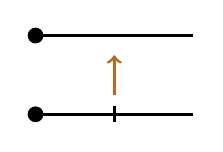
\begin{tikzpicture}[line width=1pt]
\fill (0,0) circle (.1);
\draw (0,0) -- (2,0);
\draw (1,0.1) -- (1,-0.1);

\draw [->, arcolor] (1,0.25) -- (1,0.75);

\fill (0,1) circle (.1);
\draw (0,1) -- (2,1);
\end{tikzpicture}
\qquad
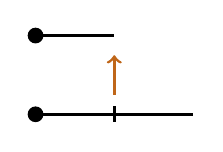
\begin{tikzpicture}[line width=1pt]
\fill (0,0) circle (.1);
\draw (0,0) -- (2,0);
\draw (1,0.1) -- (1,-0.1);

\draw [->, arcolor] (1,0.25) -- (1,0.75);

\fill (0,1) circle (.1);
\draw (0,1) -- (1,1);
\end{tikzpicture}
\qquad
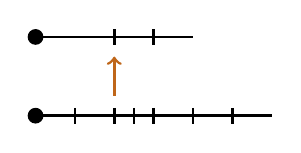
\begin{tikzpicture}[line width=1pt]
\fill (0,0) circle (.1);
\draw (0,0) -- (3,0);
\foreach \x in {0.5, 1.0, 1.25, 1.5, 2.0, 2.5} {
	\draw (\x,0.1) -- (\x,-0.1);
}

\draw [->, arcolor] (1,0.25) -- (1,0.75);

\fill (0,1) circle (.1);
\draw (0,1) -- (2,1);
\foreach \x in {1.0, 1.5} {
	\draw (\x,1.1) -- (\x,0.9);
}

\end{tikzpicture}
$$
\caption{Antirefinements of left-marked intervals}\label{fig:lmar}\end{figure}

Now we define the chain complex $\hom_\cC(\cX_\cC \to \cY_\cC)$.
The underlying vector space is 
\[
	\prod_l \prod_{\olD} \hom[l]\left(
				\cX(I_1)\ot\cC(I_2)\ot\cdots\ot\cC(I_{p-1}) \to 
							\cY(I_1\cup\cdots\cup I_{p-1}) \rule{0pt}{1.1em}\right) ,
\]
where, as usual $\olD = (D_0\cdots D_l)$ is a chain of antirefinements
(but now of left-marked intervals) and $D_0$ is the subdivision $I_1\cup\cdots\cup I_{p-1}$.
$\hom[l](- \to -)$ means graded linear maps of degree $l$.

\nn{small issue (pun intended): 
the above is a vector space only if the class of subdivisions is a set, e.g. only if
all of our left-marked intervals are contained in some universal interval (like $J$ above).
perhaps we should give another version of the definition in terms of natural transformations of functors.}

Abusing notation slightly, we will denote elements of the above space by $g$, with
\[
	\olD\ot x \ot \cbar \mapsto g(\olD\ot x \ot \cbar) \in \cY(I_1\cup\cdots\cup I_{p-1}) .
\]
For fixed $D_0$ and $D_1$, let $\cbar = \cbar'\ot\cbar''$, 
where $\cbar'$ corresponds to the subintervals of $D_0$ which map to $D_1$ and 
$\cbar''$ corresponds to the subintervals
which are dropped off the right side.
(If no such subintervals are dropped, then $\cbar''$ is empty.)
Translating from the boundary map for $(\cM_\cC\ot {_\cC\cN})^*$  appearing in Equation \eqref{eq:tensor-product-boundary},
we have
\begin{eqnarray*}
	(\bd g)(\olD\ot x \ot \cbar) &=& \bd(g(\olD\ot x \ot \cbar)) + g(\olD\ot\bd(x\ot\cbar)) + \\
	& & \;\; g((\bd_+\olD)\ot x\ot\cbar) + \gl''(g((\bd_0\olD)\ot \gl'(x\ot\cbar'))\ot\cbar'') .
\end{eqnarray*}
\nn{put in signs, rearrange terms to match order in previous formulas}
Here $\gl''$ denotes the module action in $\cY_\cC$
and $\gl'$ denotes the module action in $\cX_\cC$.
This completes the definition of $\hom_\cC(\cX_\cC \to \cY_\cC)$.

Note that if $\bd g = 0$, then each 
\[
	g(\olD\ot -) : \cX(I_1)\ot\cC(I_2)\ot\cdots\ot\cC(I_{p-1}) \to \cY(I_1\cup\cdots\cup I_{p-1})
\]
constitutes a null homotopy of
$g((\bd \olD)\ot -)$ (where the $g((\bd_0 \olD)\ot -)$ part of $g((\bd \olD)\ot -)$
should be interpreted as above).

Define a {\it strong morphism} 
of modules to be a collection of {\it chain} maps
\[
	h_K : \cX(K)\to \cY(K)
\]
for each left-marked interval $K$.
These are required to commute with gluing;
for each subdivision $K = I_1\cup\cdots\cup I_q$ the following diagram commutes:
\[ \xymatrix{
	\cX(I_1)\ot\cC(I_2)\ot\cdots\ot\cC(I_q) \ar[r]^{h_{I_0}\ot \id} 
							\ar[d]_{\gl} & \cY(I_1)\ot\cC(I_2)\ot\cdots\ot\cC(I_q) 
								\ar[d]^{\gl} \\
	\cX(K) \ar[r]^{h_{K}} & \cY(K)
} \]
Given such an $h$ we can construct a morphism $g$, with $\bd g = 0$, as follows.
Define $g(\olD\ot - ) = 0$ if the length/degree of $\olD$ is greater than 0.
If $\olD$ consists of the single subdivision $K = I_0\cup\cdots\cup I_q$ then define
\[
	g(\olD\ot x\ot \cbar) \deq h_K(\gl(x\ot\cbar)) .
\]
Trivially, we have $(\bd g)(\olD\ot x \ot \cbar) = 0$ if $\deg(\olD) > 1$.
If $\deg(\olD) = 1$, $(\bd g) = 0$ is equivalent to the fact that $h$ commutes with gluing.
If $\deg(\olD) = 0$, $(\bd g) = 0$ is equivalent to the fact 
that each $h_K$ is a chain map.

We can think of a general closed element $g\in \hom_\cC(\cX_\cC \to \cY_\cC)$
as a collection of chain maps which commute with the module action (gluing) up to coherent homotopy.
\nn{ideally should give explicit examples of this in low degrees, 
but skip that for now.}
\nn{should also say something about composition of morphisms; well-defined up to homotopy, or maybe
should make some arbitrary choice}
\medskip

Given $_\cC\cZ$ and  $g: \cX_\cC \to \cY_\cC$ with $\bd g = 0$ as above, we next define a chain map
\[
	g\ot\id : \cX_\cC \ot {}_\cC\cZ \to \cY_\cC \ot {}_\cC\cZ .
\]
\nn{...}
More generally, we have a chain map
\[
	\hom_\cC(\cX_\cC \to \cY_\cC) \ot \cX_\cC \ot {}_\cC\cZ \to \cY_\cC \ot {}_\cC\cZ .
\]

\nn{not sure whether to do low degree examples or try to state the general case; ideally both,
but maybe just low degrees for now.}


\nn{...}


\medskip


%\nn{should we define functors between $n$-cats in a similar way?  i.e.\ natural transformations
%of the $\cC$ functors which commute with gluing only up to higher morphisms?
%perhaps worth having both definitions available.
%certainly the simple kind (strictly commute with gluing) arise in nature.}




\subsection{The $n{+}1$-category of sphere modules}
\label{ssec:spherecat}

In this subsection we define $n{+}1$-categories $\cS$ of ``sphere modules" 
whose objects are $n$-categories.
With future applications in mind, we treat simultaneously the big category
of all $n$-categories and all sphere modules and also subcategories thereof.
When $n=1$ this is closely related to familiar $2$-categories consisting of 
algebras, bimodules and intertwiners (or a subcategory of that).

While it is appropriate to call an $S^0$ module a bimodule,
this is much less true for higher dimensional spheres, 
so we prefer the term ``sphere module" for the general case.

%The results of this subsection are not needed for the rest of the paper,
%so we will skimp on details in a couple of places. We have included this mostly 
%for the sake of comparing our notion of a topological $n$-category to other definitions.

For simplicity, we will assume that $n$-categories are enriched over $\c$-vector spaces.

The $0$- through $n$-dimensional parts of $\cS$ are various sorts of modules, and we describe
these first.
The $n{+}1$-dimensional part of $\cS$ consists of intertwiners
of  $1$-category modules associated to decorated $n$-balls.
We will see below that in order for these $n{+}1$-morphisms to satisfy all of
the axioms of an $n{+}1$-category (in particular, duality requirements), we will have to assume
that our $n$-categories and modules have non-degenerate inner products.
(In other words, we need to assume some extra duality on the $n$-categories and modules.)

\medskip

Our first task is to define an $n$-category $m$-sphere module, for $0\le m \le n-1$.
These will be defined in terms of certain classes of marked balls, very similarly
to the definition of $n$-category modules above.
(This, in turn, is very similar to our definition of $n$-category.)
Because of this similarity, we only sketch the definitions below.

We start with $0$-sphere modules, which also could reasonably be called (categorified) bimodules.
(For $n=1$ they are precisely bimodules in the usual, uncategorified sense.)
We prefer the more awkward term ``0-sphere module" to emphasize the analogy
with the higher sphere modules defined below.

Define a $0$-marked $k$-ball, $1\le k \le n$, to be a pair  $(X, M)$ homeomorphic to the standard
$(B^k, B^{k-1})$.
See Figure \ref{feb21a}.
Another way to say this is that $(X, M)$ is homeomorphic to $B^{k-1}\times([-1,1], \{0\})$.

\begin{figure}[t]
$$\tikz[baseline,line width=2pt]{\draw[blue] (-2,0)--(2,0); \fill[red] (0,0) circle (0.1);} \qquad \qquad \tikz[baseline,line width=2pt]{\draw[blue][fill=blue!30!white] (0,0) circle (2 and 1); \draw[red] (0,1)--(0,-1);}$$
\caption{0-marked 1-ball and 0-marked 2-ball}
\label{feb21a}
\end{figure}

The $0$-marked balls can be cut into smaller balls in various ways.
We only consider those decompositions in which the smaller balls are either
$0$-marked (i.e. intersect the $0$-marking of the large ball in a disc) 
or plain (don't intersect the $0$-marking of the large ball).
We can also take the boundary of a $0$-marked ball, which is $0$-marked sphere.

Fix $n$-categories $\cA$ and $\cB$.
These will label the two halves of a $0$-marked $k$-ball.

An $n$-category $0$-sphere module $\cM$ over the $n$-categories $\cA$ and $\cB$ is a collection of functors $\cM_k$ from the category
of $0$-marked $k$-balls, $1\le k \le n$,
(with the two halves labeled by $\cA$ and $\cB$) to the category of sets.
If $k=n$ these sets should be enriched to the extent $\cA$ and $\cB$ are.
Given a decomposition of a $0$-marked $k$-ball $X$ into smaller balls $X_i$, we have
morphism sets $\cA_k(X_i)$ (if $X_i$ lies on the $\cA$-labeled side)
or $\cB_k(X_i)$ (if $X_i$ lies on the $\cB$-labeled side)
or $\cM_k(X_i)$ (if $X_i$ intersects the marking and is therefore a smaller 0-marked ball).
Corresponding to this decomposition we have a composition (or ``gluing") map
from the product (fibered over the boundary data) of these various sets into $\cM_k(X)$.

\medskip

Part of the structure of an $n$-category 0-sphere module $\cM$  is captured by saying it is
a collection $\cD^{ab}$ of $n{-}1$-categories, indexed by pairs $(a, b)$ of objects (0-morphisms)
of $\cA$ and $\cB$.
Let $J$ be some standard 0-marked 1-ball (i.e.\ an interval with a marked point in its interior).
Given a $j$-ball $X$, $0\le j\le n-1$, we define
\[
	\cD(X) \deq \cM(X\times J) .
\]
The product is pinched over the boundary of $J$.
The set $\cD$ breaks into ``blocks" according to the restrictions to the pinched points of $X\times J$
(see Figure \ref{feb21b}).
These restrictions are 0-morphisms $(a, b)$ of $\cA$ and $\cB$.

\begin{figure}[t]
$$
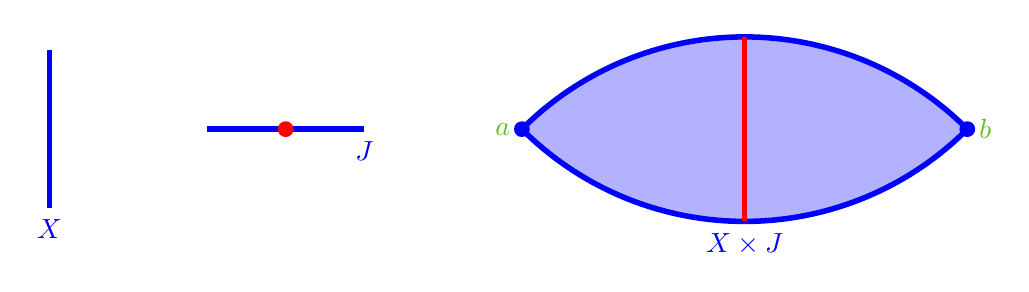
\begin{tikzpicture}[blue,line width=2pt]
\draw (0,1) -- (0,-1) node[below] {$X$};

\draw (2,0) -- (4,0) node[below] {$J$};
\fill[red] (3,0) circle (0.1);

\draw[fill=blue!30!white] (6,0) node(a) {} arc (135:90:4) node(top) {} arc (90:45:4) node(b) {} arc (-45:-90:4) node(bottom) {} arc(-90:-135:4);
\draw[red] (top.center) -- (bottom.center);
\fill (a) circle (0.1) node[left] {\color{green!50!brown} $a$};
\fill (b) circle (0.1) node[right] {\color{green!50!brown} $b$};

\path (bottom) node[below]{$X \times J$};

\end{tikzpicture}
$$
\caption{The pinched product $X\times J$}
\label{feb21b}
\end{figure}

More generally, consider an interval with interior marked points, and with the complements
of these points labeled by $n$-categories $\cA_i$ ($0\le i\le l$) and the marked points labeled
by $\cA_i$-$\cA_{i+1}$ 0-sphere modules $\cM_i$.
(See Figure \ref{feb21c}.)
To this data we can apply the coend construction as in \S\ref{moddecss} above
to obtain an $\cA_0$-$\cA_l$ $0$-sphere module and, forgetfully, an $n{-}1$-category.
This amounts to a definition of taking tensor products of $0$-sphere modules over $n$-categories.

\begin{figure}[t]
$$
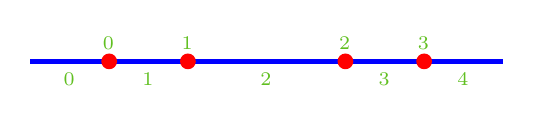
\begin{tikzpicture}[baseline,line width = 2pt]
\draw[blue] (0,0) -- (6,0);
\foreach \x/\n in {0.5/0,1.5/1,3/2,4.5/3,5.5/4} {
	\path (\x,0)  node[below] {\color{green!50!brown}$\cA_{\n}$};
}
\foreach \x/\n in {1/0,2/1,4/2,5/3} {
	\fill[red] (\x,0) circle (0.1) node[above] {\color{green!50!brown}$\cM_{\n}$};
}
\end{tikzpicture}
\qquad
\qquad
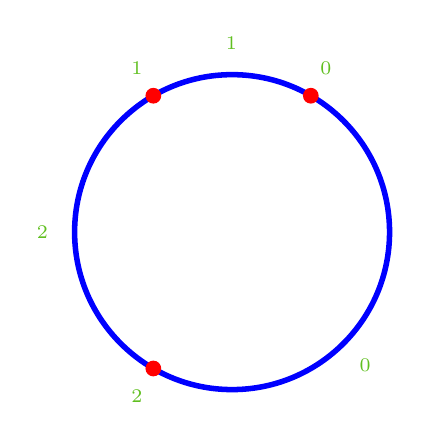
\begin{tikzpicture}[baseline,line width = 2pt]
\draw[blue] (0,0) circle (2);
\foreach \q/\n in {-45/0,90/1,180/2} {
	\path (\q:2.4)  node {\color{green!50!brown}$\cA_{\n}$};
}
\foreach \q/\n in {60/0,120/1,-120/2} {
	\fill[red] (\q:2) circle (0.1);
	\path (\q:2.4) node {\color{green!50!brown}$\cM_{\n}$};
}
\end{tikzpicture}
$$
\caption{Marked and labeled 1-manifolds}
\label{feb21c}
\end{figure}

We could also similarly mark and label a circle, obtaining an $n{-}1$-category
associated to the marked and labeled circle.
(See Figure \ref{feb21c}.)
If the circle is divided into two intervals, we can think of this $n{-}1$-category
as the 2-sided tensor product of the two 0-sphere modules associated to the two intervals.

\medskip

Next we define $n$-category 1-sphere modules.
These are just representations of (modules for) $n{-}1$-categories associated to marked and labeled 
circles (1-spheres) which we just introduced.

Equivalently, we can define 1-sphere modules in terms of 1-marked $k$-balls, $2\le k\le n$.
Fix a marked (and labeled) circle $S$.
Let $C(S)$ denote the cone of $S$, a marked 2-ball (Figure \ref{feb21d}).
%\nn{I need to make up my mind whether marked things are always labeled too.
%For the time being, let's say they are.}
A 1-marked $k$-ball is anything homeomorphic to $B^j \times C(S)$, $0\le j\le n-2$, 
where $B^j$ is the standard $j$-ball.
A 1-marked $k$-ball can be decomposed in various ways into smaller balls, which are either 
(a) smaller 1-marked $k$-balls, (b) 0-marked $k$-balls, or (c) plain $k$-balls.
(See Figure \nn{need figure}.)
We now proceed as in the above module definitions.

\begin{figure}[!ht]
$$
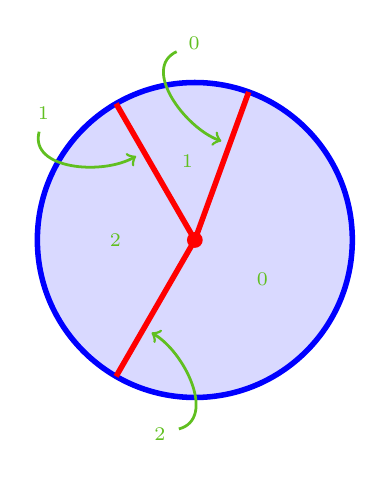
\begin{tikzpicture}[baseline,line width = 2pt]
\draw[blue][fill=blue!15!white] (0,0) circle (2);
\fill[red] (0,0) circle (0.1);
\foreach \qm/\qa/\n in {70/-30/0, 120/95/1, -120/180/2} {
	\draw[red] (0,0) -- (\qm:2);
	\path (\qa:1) node {\color{green!50!brown} $\cA_\n$};
	\path (\qm+20:2.5) node(M\n) {\color{green!50!brown} $\cM_\n$};
	\draw[line width=1pt, green!50!brown, ->] (M\n.\qm+135) to[out=\qm+135,in=\qm+90] (\qm+5:1.3);
}
\end{tikzpicture}
$$
\caption{Cone on a marked circle}
\label{feb21d}
\end{figure}

A $n$-category 1-sphere module is, among other things, an $n{-}2$-category $\cD$ with
\[
	\cD(X) \deq \cM(X\times C(S)) .
\]
The product is pinched over the boundary of $C(S)$.
$\cD$ breaks into ``blocks" according to the restriction to the 
image of $\bd C(S) = S$ in $X\times C(S)$.

More generally, consider a 2-manifold $Y$ 
(e.g.\ 2-ball or 2-sphere) marked by an embedded 1-complex $K$.
The components of $Y\setminus K$ are labeled by $n$-categories, 
the edges of $K$ are labeled by 0-sphere modules, 
and the 0-cells of $K$ are labeled by 1-sphere modules.
We can now apply the coend construction and obtain an $n{-}2$-category.
If $Y$ has boundary then this $n{-}2$-category is a module for the $n{-}1$-category
associated to the (marked, labeled) boundary of $Y$.
In particular, if $\bd Y$ is a 1-sphere then we get a 1-sphere module as defined above.

\medskip

It should now be clear how to define $n$-category $m$-sphere modules for $0\le m \le n-1$.
For example, there is an $n{-}2$-category associated to a marked, labeled 2-sphere,
and a 2-sphere module is a representation of such an $n{-}2$-category.

\medskip

We can now define the $n$-or-less-dimensional part of our $n{+}1$-category $\cS$.
Choose some collection of $n$-categories, then choose some collections of 0-sphere modules between
these $n$-categories, then choose some collection of 1-sphere modules for the various
possible marked 1-spheres labeled by the $n$-categories and 0-sphere modules, and so on.
Let $L_i$ denote the collection of $i{-}1$-sphere modules we have chosen.
(For convenience, we declare a $(-1)$-sphere module to be an $n$-category.)
There is a wide range of possibilities.
The set $L_0$ could contain infinitely many $n$-categories or just one.
For each pair of $n$-categories in $L_0$, $L_1$ could contain no 0-sphere modules at all or 
it could contain several.
The only requirement is that each $k$-sphere module be a module for a $k$-sphere $n{-}k$-category
constructed out of labels taken from $L_j$ for $j<k$.

We now define $\cS(X)$, for $X$ a ball of dimension at most $n$, to be the set of all 
cell-complexes $K$ embedded in $X$, with the codimension-$j$ parts of $(X, K)$ labeled
by elements of $L_j$.
As described above, we can think of each decorated $k$-ball as defining a $k{-}1$-sphere module
for the $n{-}k{+}1$-category associated to its decorated boundary.
Thus the $k$-morphisms of $\cS$ (for $k\le n$) can be thought 
of as $n$-category $k{-}1$-sphere modules 
(generalizations of bimodules).
On the other hand, we can equally well think of the $k$-morphisms as decorations on $k$-balls, 
and from this point of view it is clear that they satisfy all of the axioms of an
$n{+}1$-category.
(All of the axioms for the less-than-$n{+}1$-dimensional part of an $n{+}1$-category, that is.)

\medskip

Next we define the $n{+}1$-morphisms of $\cS$.
The construction of the 0- through $n$-morphisms was easy and tautological, but the 
$n{+}1$-morphisms will require some effort and combinatorial topology, as well as additional
duality assumptions on the lower morphisms. These are required because we define the spaces of $n{+}1$-morphisms by making arbitrary choices of incoming and outgoing boundaries for each $n$-ball. The additional duality assumptions are needed to prove independence of our definition form these choices.

Let $X$ be an $n{+}1$-ball, and let $c$ be a decoration of its boundary
by a cell complex labeled by 0- through $n$-morphisms, as above.
Choose an $n{-}1$-sphere $E\sub \bd X$ which divides
$\bd X$ into ``incoming" and ``outgoing" boundary $\bd_-X$ and $\bd_+X$.
Let $E_c$ denote $E$ decorated by the restriction of $c$ to $E$.
Recall from above the associated 1-category $\cS(E_c)$.
We can also have $\cS(E_c)$ modules $\cS(\bd_-X_c)$ and $\cS(\bd_+X_c)$.
Define
\[
	\cS(X; c; E) \deq \hom_{\cS(E_c)}(\cS(\bd_-X_c), \cS(\bd_+X_c)) .
\]

We will show that if the sphere modules are equipped with a ``compatible family of 
non-degenerate inner products", then there is a coherent family of isomorphisms
$\cS(X; c; E) \cong \cS(X; c; E')$ for all pairs of choices $E$ and $E'$.
This will allow us to define $\cS(X; c)$ independently of the choice of $E$.
\nn{also need to (simultaneously) show compatibility with action of homeos of boundary}

First we must define ``inner product", ``non-degenerate" and ``compatible".
Let $Y$ be a decorated $n$-ball, and $\ol{Y}$ it's mirror image.
(We assume we are working in the unoriented category.)
Let $Y\cup\ol{Y}$ denote the decorated $n$-sphere obtained by gluing $Y$ and $\ol{Y}$
along their common boundary.
An {\it inner product} on $\cS(Y)$ is a dual vector
\[
	z_Y : \cS(Y\cup\ol{Y}) \to \c.
\]
We will also use the notation
\[
	\langle a, b\rangle \deq z_Y(a\bullet \ol{b}) \in \c .
\]
An inner product induces a linear map
\begin{eqnarray*}
	\varphi: \cS(Y) &\to& \cS(Y)^* \\
	a &\mapsto& \langle a, \cdot \rangle
\end{eqnarray*}
which satisfies, for all morphisms $e$ of $\cS(\bd Y)$,
\[
	\varphi(ae)(b) = \langle ae, b \rangle = z_Y(a\bullet e\bullet b) = 
			\langle a, eb \rangle = \varphi(a)(eb) .
\]
In other words, $\varphi$ is a map of $\cS(\bd Y)$ modules.
An inner product is {\it non-degenerate} if $\varphi$ is an isomorphism.
This implies that $\cS(Y; c)$ is finite dimensional for all boundary conditions $c$.
(One can think of these inner products as giving some duality in dimension $n{+}1$;
heretofore we have only assumed duality in dimensions 0 through $n$.)

Next we define compatibility.
Let $Y = Y_1\cup Y_2$ with $D = Y_1\cap Y_2$.
Let $X_1$ and $X_2$ be the two components of $Y\times I$ cut along
$D\times I$, in both cases using the pinched product.
(Here we are overloading notation and letting $D$ denote both a decorated and an undecorated
manifold.)
We have $\bd X_i = Y_i \cup \ol{Y}_i \cup (D\times I)$
(see Figure \ref{jun23a}).
\begin{figure}[t]
\begin{equation*}
\mathfig{.6}{tempkw/jun23a}
\end{equation*}
\caption{$Y\times I$ sliced open}
\label{jun23a}
\end{figure}
Given $a_i\in \cS(Y_i)$, $b_i\in \cS(\ol{Y}_i)$ and $v\in\cS(D\times I)$
which agree on their boundaries, we can evaluate
\[
	z_{Y_i}(a_i\bullet b_i\bullet v) \in \c .
\]
(This requires a choice of homeomorphism $Y_i \cup \ol{Y}_i \cup (D\times I) \cong
Y_i \cup \ol{Y}_i$, but the value of $z_{Y_i}$ is independent of this choice.)
We can think of $z_{Y_i}$ as giving a function
\[
	\psi_i : \cS(Y_i) \ot \cS(\ol{Y}_i) \to \cS(D\times I)^* 
					\stackrel{\varphi\inv}{\longrightarrow} \cS(D\times I) .
\]
We can now finally define a family of inner products to be {\it compatible} if
for all decompositions $Y = Y_1\cup Y_2$ as above and all $a_i\in \cS(Y_i)$, $b_i\in \cS(\ol{Y}_i)$
we have
\[
	z_Y(a_1\bullet a_2\bullet b_1\bullet b_2) = 
				z_{D\times I}(\psi_1(a_1\ot b_1)\bullet \psi_2(a_2\ot b_2)) .
\]
In other words, the inner product on $Y$ is determined by the inner products on
$Y_1$, $Y_2$ and $D\times I$.

Now we show how to unambiguously identify $\cS(X; c; E)$ and $\cS(X; c; E')$ for any
two choices of $E$ and $E'$.
Consider first the case where $\bd X$ is decomposed as three $n$-balls $A$, $B$ and $C$,
with $E = \bd(A\cup B)$ and $E' = \bd A$.
We must provide an isomorphism between $\cS(X; c; E) = \hom(\cS(C), \cS(A\cup B))$
and $\cS(X; c; E') = \hom(\cS(C\cup \ol{B}), \cS(A))$.
Let $D = B\cap A$.
Then as above we can construct a map
\[
	\psi: \cS(B)\ot\cS(\ol{B}) \to \cS(D\times I) .
\]
Given $f\in \hom(\cS(C), \cS(A\cup B))$ we define $f'\in \hom(\cS(C\cup \ol{B}), \cS(A))$
to be the composition
\[
	\cS(C\cup \ol{B}) \stackrel{f\ot\id}{\longrightarrow}
		\cS(A\cup B\cup \ol{B})  \stackrel{\id\ot\psi}{\longrightarrow}
			\cS(A\cup(D\times I)) \stackrel{\cong}{\longrightarrow} \cS(A) .
\]
(See Figure \ref{jun23b}.)
\begin{figure}[t]
$$
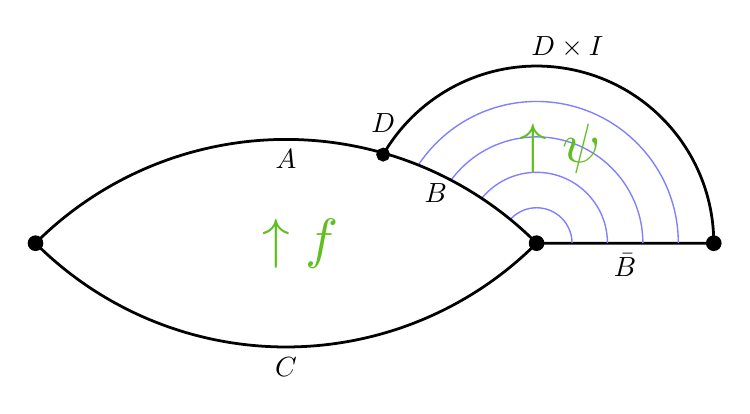
\begin{tikzpicture}[baseline,line width = 1pt,x=1.5cm,y=1.5cm]
\draw (0,0) node(R) {}
	-- (0.75,0) node[below] {$\bar{B}$}
	--(1.5,0)  node[circle,fill=black,inner sep=2pt] {}
	arc (0:80:1.5) node[above] {$D \times I$}
	arc (80:180:1.5);
\foreach \r in {0.3, 0.6, 0.9, 1.2} {
	\draw[blue!50, line width = 0.5pt] (\r,0) arc (0:180:\r);
}
\draw[fill=white]
	(R) node[circle,fill=black,inner sep=2pt] {}
	arc (45:65:3) node[below] {$B$}
	arc (65:90:3) node[below] {$A$}
	arc (90:135:3) node[circle,fill=black,inner sep=2pt] {}
	arc (-135:-90:3) node[below] {$C$}
	arc (-90:-45:3);
\draw[fill]  (150:1.5) circle (2pt) node[above=4pt] {$D$};
\node[green!50!brown] at (-2,0) {\scalebox{2.0}{$\uparrow f$}};
\node[green!50!brown] at (0.2,0.8) {\scalebox{2.0}{$\uparrow \psi$}};
\end{tikzpicture}
$$
\caption{Moving $B$ from top to bottom}
\label{jun23b}
\end{figure}
Let $D' = B\cap C$.
Using the inner products there is an adjoint map
\[
	\psi^\dagger: \cS(D'\times I) \to \cS(\ol{B})\ot\cS(B) .
\]
Given $f'\in \hom(\cS(C\cup \ol{B}), \cS(A))$ we define $f\in \hom(\cS(C), \cS(A\cup B))$
to be the composition
\[
	\cS(C) \stackrel{\cong}{\longrightarrow}
		\cS(C\cup(D'\times I)) \stackrel{\id\ot\psi^\dagger}{\longrightarrow}
			\cS(C\cup \ol{B}\cup B)   \stackrel{f'\ot\id}{\longrightarrow}
				\cS(A\cup B) .
\]
(See Figure \ref{jun23c}.)
\begin{figure}[t]
\begin{equation*}
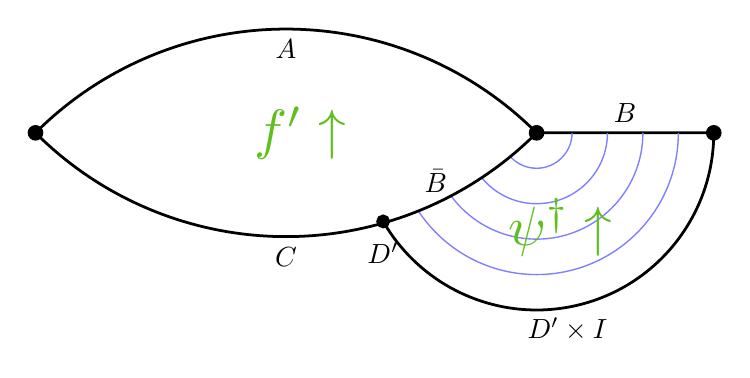
\begin{tikzpicture}[baseline,line width = 1pt,x=1.5cm,y=-1.5cm]
\draw (0,0) node(R) {}
	-- (0.75,0) node[above] {$B$}
	--(1.5,0)  node[circle,fill=black,inner sep=2pt] {}
	arc (0:80:1.5) node[below] {$D' \times I$}
	arc (80:180:1.5);
\foreach \r in {0.3, 0.6, 0.9, 1.2} {
	\draw[blue!50, line width = 0.5pt] (\r,0) arc (0:180:\r);
}
\draw[fill=white]
	(R) node[circle,fill=black,inner sep=2pt] {}
	arc (45:65:3) node[above] {$\bar{B}$}
	arc (65:90:3) node[below] {$C$}
	arc (90:135:3) node[circle,fill=black,inner sep=2pt] {}
	arc (-135:-90:3) node[below] {$A$}
	arc (-90:-45:3);
\draw[fill]  (150:1.5) circle (2pt) node[below=4pt] {$D'$};
\node[green!50!brown] at (-2,0) {\scalebox{2.0}{$f'\uparrow $}};
\node[green!50!brown] at (0.2,0.8) {\scalebox{2.0}{$\psi^\dagger \uparrow $}};
\end{tikzpicture}
\end{equation*}
\caption{Moving $B$ from bottom to top}
\label{jun23c}
\end{figure}
Let $D' = B\cap C$.
It is not hard too show that the above two maps are mutually inverse.

\begin{lem}
Any two choices of $E$ and $E'$ are related by a series of modifications as above.
\end{lem}

\begin{proof}
(Sketch)
$E$ and $E'$ are isotopic, and any isotopy is 
homotopic to a composition of small isotopies which are either
(a) supported away from $E$, or (b) modify $E$ in the simple manner described above.
\end{proof}

It follows from the lemma that we can construct an isomorphism
between $\cS(X; c; E)$ and $\cS(X; c; E')$ for any pair $E$, $E'$.
This construction involves on a choice of simple ``moves" (as above) to transform
$E$ to $E'$.
We must now show that the isomorphism does not depend on this choice.
We will show below that it suffice to check three ``movie moves".

The first movie move is to push $E$ across an $n$-ball $B$ as above, then push it back.
The result is equivalent to doing nothing.
As we remarked above, the isomorphisms corresponding to these two pushes are mutually
inverse, so we have invariance under this movie move.

The second movie move replaces two successive pushes in the same direction,
across $B_1$ and $B_2$, say, with a single push across $B_1\cup B_2$.
(See Figure \ref{jun23d}.)
\begin{figure}[t]
\begin{tikzpicture}
\node(L) {
\scalebox{0.5}{
\begin{tikzpicture}[baseline,line width = 1pt,x=1.5cm,y=1.5cm]
\draw[red] (0.75,0) -- +(2,0);
\draw[red] (0,0) node(R) {}
	-- (0.75,0) node[below] {}
	--(1.5,0)  node[circle,fill=black,inner sep=2pt] {};
\draw[fill]  (150:1.5) circle (2pt) node[above=4pt] {};
\draw (1.5,0) arc (0:149:1.5);
\draw[red]
	(R) node[circle,fill=black,inner sep=2pt] {}
	arc (-45:-135:3) node[circle,fill=black,inner sep=2pt] {};
\draw[red] (-5.5,0) -- (-4.2,0);
\draw (R) arc (45:75:3);
\draw (150:1.5) arc (74:135:3);
\node at (-2,0) {\scalebox{2.0}{$B_1$}};
\node at (0.2,0.8) {\scalebox{2.0}{$B_2$}};
\node at (-4,1.2) {\scalebox{2.0}{$A$}};
\node at (-4,-1.2) {\scalebox{2.0}{$C$}};
\node[red] at (2.53,0.35) {\scalebox{2.0}{$E$}};
\end{tikzpicture}
}
};
\node(M) at (5,4) {
\scalebox{0.5}{
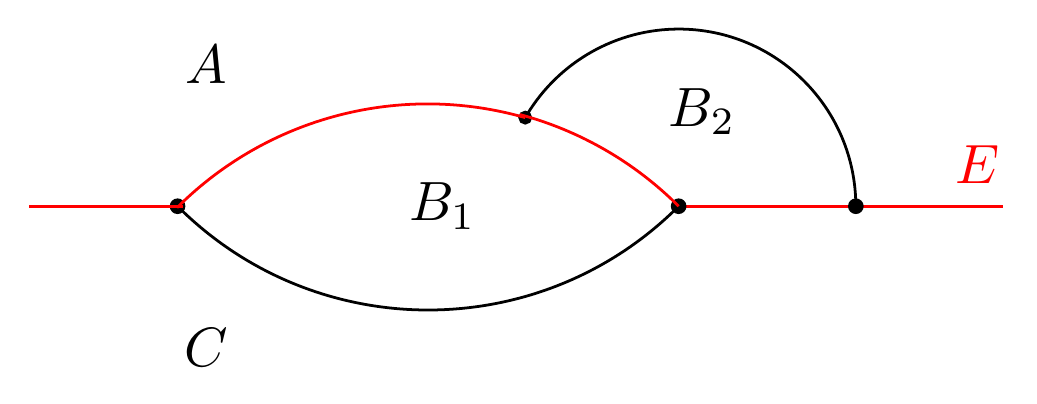
\begin{tikzpicture}[baseline,line width = 1pt,x=1.5cm,y=1.5cm]
\draw[red] (0.75,0) -- +(2,0);
\draw[red] (0,0) node(R) {}
	-- (0.75,0) node[below] {}
	--(1.5,0)  node[circle,fill=black,inner sep=2pt] {};
\draw[fill]  (150:1.5) circle (2pt) node[above=4pt] {};
\draw(1.5,0) arc (0:149:1.5);
\draw
	(R) node[circle,fill=black,inner sep=2pt] {}
	arc (-45:-135:3) node[circle,fill=black,inner sep=2pt] {};
\draw[red] (-5.5,0) -- (-4.2,0);
\draw[red] (R) arc (45:75:3);
\draw[red] (150:1.5) arc (74:135:3);
\node at (-2,0) {\scalebox{2.0}{$B_1$}};
\node at (0.2,0.8) {\scalebox{2.0}{$B_2$}};
\node at (-4,1.2) {\scalebox{2.0}{$A$}};
\node at (-4,-1.2) {\scalebox{2.0}{$C$}};
\node[red] at (2.53,0.35) {\scalebox{2.0}{$E$}};
\end{tikzpicture}
}
};
\node(R) at (10,0) {
\scalebox{0.5}{
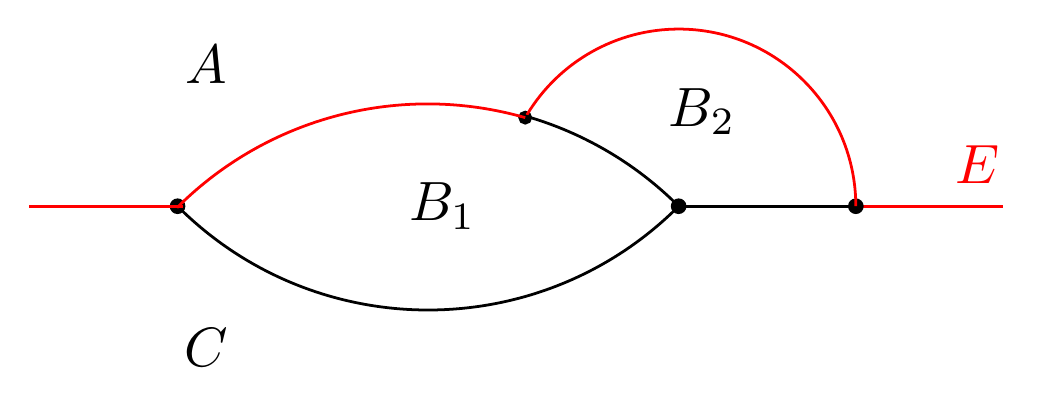
\begin{tikzpicture}[baseline,line width = 1pt,x=1.5cm,y=1.5cm]
\draw[red] (0.75,0) -- +(2,0);
\draw (0,0) node(R) {}
	-- (0.75,0) node[below] {}
	--(1.5,0)  node[circle,fill=black,inner sep=2pt] {};
\draw[fill]  (150:1.5) circle (2pt) node[above=4pt] {};
\draw[red] (1.5,0) arc (0:149:1.5);
\draw
	(R) node[circle,fill=black,inner sep=2pt] {}
	arc (-45:-135:3) node[circle,fill=black,inner sep=2pt] {};
\draw[red] (-5.5,0) -- (-4.2,0);
\draw (R) arc (45:75:3);
\draw[red] (150:1.5) arc (74:135:3);
\node at (-2,0) {\scalebox{2.0}{$B_1$}};
\node at (0.2,0.8) {\scalebox{2.0}{$B_2$}};
\node at (-4,1.2) {\scalebox{2.0}{$A$}};
\node at (-4,-1.2) {\scalebox{2.0}{$C$}};
\node[red] at (2.53,0.35) {\scalebox{2.0}{$E$}};
\end{tikzpicture}
}
};
\draw[->] (L) to[out=90,in=225] node[sloped, above] {push $B_1$} (M);
\draw[->] (M)  to[out=-45,in=90] node[sloped, above] {push $B_2$} (R);
\draw[->] (L) to[out=-35,in=-145] node[sloped, below] {push $B_1 \cup B_2$} (R);
\end{tikzpicture}
\caption{A movie move}
\label{jun23d}
\end{figure}
Invariance under this movie move follows from the compatibility of the inner
product for $B_1\cup B_2$ with the inner products for $B_1$ and $B_2$.

The third movie move could be called ``locality" or ``disjoint commutativity".
\nn{...}

If $n\ge 2$, these three movie move suffice:

\begin{lem}
Assume $n\ge 2$ and fix $E$ and $E'$ as above.
The any two sequences of elementary moves connecting $E$ to $E'$
are related by a sequence of the three movie moves defined above.
\end{lem}

\begin{proof}
(Sketch)
Consider a two parameter family of diffeomorphisms (one parameter family of isotopies) 
of $\bd X$.
Up to homotopy,
such a family is homotopic to a family which can be decomposed 
into small families which are either
(a) supported away from $E$, 
(b) have boundaries corresponding to the three movie moves above.
Finally, observe that the space of $E$'s is simply connected.
(This fails for $n=1$.)
\end{proof}

For $n=1$ we have to check an additional ``global" relations corresponding to 
rotating the 0-sphere $E$ around the 1-sphere $\bd X$.
\nn{should check this global move, or maybe cite Frobenius reciprocity result}

\nn{...}

\medskip
\hrule
\medskip

\nn{to be continued...}
\medskip






Stuff that remains to be done (either below or in an appendix or in a separate section or in
a separate paper):
\begin{itemize}
\item discuss Morita equivalence
\item functors
\end{itemize}


